% ============================================================
%  OUP version (Digital Scholarship in the Humanities)
%  Compile: pdflatex → bibtex → pdflatex → pdflatex
% ============================================================
\documentclass[numsec,webpdf,modern,medium,namedate]{oup-authoring-template}

\graphicspath{{../images/}{../}}

% --- Mathematics ---
\usepackage{amsmath,amssymb}

% --- Tables ---
\usepackage{booktabs}
\usepackage{multirow}
\usepackage{tabularx}
\usepackage{adjustbox}

% --- Misc ---
\usepackage{enumitem}

% --- Typography ---
\usepackage{microtype}
\emergencystretch=1em

% --- Custom commands ---
\newcommand{\vms}{Voynich Manuscript}
\newcommand{\MI}{\mathrm{MI}}
\newcommand{\JSD}{\mathrm{JSD}}
\newcommand{\Rhat}{\hat{R}}

% --- OUP flag (controls table*/tabular* in shared body) ---
\newif\ifoup
\ouptrue

% ============================================================
\begin{document}

\journaltitle{Digital Scholarship in the Humanities}
\DOI{DOI HERE}
\copyrightyear{2026}
\pubyear{2026}
\access{Advance Access Publication Date: Day Month Year}
\appnotes{Paper}

\firstpage{1}

\title[Computational Analysis of the Voynich Manuscript]{Computational Analysis of the Voynich Manuscript: Statistical Fingerprinting, Generative Modelling, and Sixteen Decipherment Models Yield a Structured Negative Result}

\author[1,$\ast$]{C\'esar Jim\'enez Zapata}

\authormark{Jim\'enez Zapata}

\address[1]{\orgname{Independent Researcher}, \orgaddress{\country{Spain}}}

\corresp[$\ast$]{Corresponding author. \href{mailto:cesarjz@gmail.com}{cesarjz@gmail.com}}

\received{11}{3}{2026}

\abstract{
% Abstract text — shared across all versions
% Do not add \begin{abstract} here — the wrapper handles that

The Voynich Manuscript (Beinecke MS~408, radiocarbon-dated 1404--1438~CE) is a 234-page illustrated codex written in an unidentified script of approximately 166 distinct glyphs.  We develop a four-stage computational pipeline---statistical fingerprinting, generative model comparison, syllabic segmentation, and Bayesian decipherment---applied to the STA1~2.0 corpus (37,087 words, 157,254 glyph tokens).  The fingerprint reveals a unique U-shaped entropy curve (bounce $= 0.813$, absent from all controls) and positional mutual information (0.658~bits) twice that of any tested language.  Comparison of eleven generative models identifies a syllabic-partition mechanism (SilPart, $d = 0.445$) as the only model reproducing the full fingerprint; four published hypotheses are quantitatively eliminated.  Bayesian ranking across six candidate languages places Hebrew and Aramaic as statistically indistinguishable top candidates (gap $\sim$0.01~nats, within bootstrap CI spanning zero).  However, nineteen decipherment models---spanning trigram and neural LMs, single and triple mapping tables, character and syllable targets, morphological role indexing, and three additional cross-linguistic targets (Tibbonid Hebrew, Judeo-Arabic, Classical Ge'ez)---all converge on the same structural ceiling: approximately 68\% $n$-gram realism and 3--5 root matches at best.  No model produces readable text.  The Ge'ez experiment ($|\Sigma|/|\mathcal{A}| \approx 0.88$, the first near-1:1 test) confirms that the barrier is not an artefact of alphabet-size mismatch.  Classical cipher-type diagnostics (IC, Kasiski, bigram entropy, transposition) further exclude polyalphabetic, polygraphic, and transposition ciphers, establishing a central paradox: the text behaves statistically like natural language but resists all nineteen monoalphabetic models.  We establish quantitative falsification criteria (bounce $> 0.8$, MI$_{\text{pos}} > 0.5$) for evaluating future proposals.  The convergence of nineteen independent strategies provides strong evidence that the structural ceiling is a property of the Voynich text itself---not of any particular modelling choice---and narrows the remaining viable hypotheses to substitution to an untested language or a constructed language.  A companion study analyses the encoding mechanism directly, finding a two-tier combinatorial structure consistent with an encyclopaedic code.

}

\keywords{Voynich Manuscript, Bayesian decipherment, computational palaeography, entropy analysis, undeciphered scripts, digital humanities, structured negative result
}

\maketitle

% Body content — shared across all versions
% Included after \maketitle in each wrapper

\section{Introduction}
\label{sec:intro}

The \vms{} (Beinecke MS~408) is a 234-page illustrated codex radiocarbon-dated to 1404--1438~CE \citep{hodgins2011}, written in an unidentified script of approximately 166 distinct glyphs.  More than a century of cryptanalytic and linguistic effort has failed to produce a consensus reading \citep{dimperio1978, clemens2016}.  The manuscript's pages contain botanical illustrations, astronomical diagrams, apparent pharmaceutical recipes, and sections depicting nude female figures in pools of coloured liquid---imagery that has inspired interpretations ranging from herbal pharmacopoeia to alchemical treatise to elaborate forgery.  Proposed solutions span three categories: natural-language hypotheses mapping glyphs to known scripts \citep{stolfi1997}, constructed-language or glossolalic hypotheses \citep{rugg2004}, and meaningless-hoax theories modelling the text as output of a mechanical device \citep{rugg2004, timm2020}.

The difficulty stems from three interacting factors.  First, the 166-type alphabet is far larger than any known European writing system of the period (Latin: 26, Hebrew: 27, Arabic: 36), suggesting either a syllabary, a compositional encoding, or a cipher with extensive homophones.  Second, no bilingual text or known-plaintext crib has been identified, ruling out classical frequency-analysis approaches that have succeeded for virtually every historical cipher since Al-Kindi's 9th-century treatise \citep{kahn1967}.  Third, word-internal structure shows anomalous regularities---a near-absence of repeated bigrams and strong positional constraints on which glyphs appear at word boundaries---that have no parallel in known natural languages or historical cipher systems.

Previous computational studies have established important statistical properties.  \citet{currier1976} identified two distinct ``languages'' (A and B) through bigram statistics.  \citet{montemurro2013} showed that word-frequency distributions and long-range correlations are consistent with natural language.  \citet{amancio2013} corroborated this via complex-network analysis, showing that word co-occurrence graphs cluster with natural languages rather than with shuffled or random texts.  On the generative side, \citet{rugg2004} demonstrated that a Cardan grille produces Voynich-like tokens, while \citet{timm2020} proposed a verbose-cipher model.

Despite this progress, two fundamental gaps remain.  First, no study has compared generative hypotheses \emph{simultaneously} across a common set of diagnostic metrics, leaving the field with competing claims evaluated on incommensurable criteria.  Second, no study has attempted a \emph{unified pipeline} that proceeds from corpus-level diagnostics through generative model selection to constrained Bayesian decipherment with systematic validation.  This paper fills both gaps with a four-stage approach:

\begin{enumerate}[nosep]
  \item \textbf{Statistical fingerprinting} of the Voynich text against eight control corpora across six information-theoretic metrics.
  \item \textbf{Generative model comparison} of eleven candidate mechanisms using a weighted multi-metric distance framework.
  \item \textbf{Syllabic segmentation} via transition-probability boundaries, yielding 2,923 syllabic types.
  \item \textbf{Systematic decipherment} via nineteen distinct models against six candidate languages, evaluated with a unified five-test validation scorecard.
\end{enumerate}

Our principal finding is a \emph{structured negative result}.  The pipeline progressively narrows the hypothesis space: the fingerprint eliminates random and cipher hypotheses; generative modelling eliminates four literature proposals; Bayesian ranking identifies NW~Semitic (Hebrew/Aramaic) as the most compatible language family.  But nineteen independent decipherment strategies converge on the same structural limits---approximately 3--5 root matches and 68\% $n$-gram realism---and no model produces readable text.  We argue that this convergence elevates the negative result from methodological failure to a \emph{theoretical finding}: the Voynich script's encoding mechanism transcends monoalphabetic substitution.


% ============================================================
\section{Related Work}
\label{sec:related}

Quantitative investigation of the \vms{} began with \citet{currier1976}, who segmented the text into two statistical ``languages'' (A and B) based on digraph frequencies, establishing that the manuscript is not internally homogeneous.  \citet{stolfi1997} compiled extensive glyph statistics and identified ``crust-mantle-core'' word structure: Voynich words appear to be built from positionally constrained glyph groups.  \citet{landini2001} found evidence of periodic structure via spectral methods.  The landmark study by \citet{montemurro2013} demonstrated long-range word-frequency correlations characteristic of meaningful text, using Shannon entropy at multiple scales.  \citet{amancio2013} confirmed these findings via complex-network analysis.

More recent work has advanced both linguistic and statistical perspectives.  \citet{reddy2011} surveyed the state of computational Voynich studies, concluding that the manuscript's statistical properties are consistent with natural language but insufficient to determine its identity.  \citet{hauer2016} applied anagram-decoding techniques under the hypothesis that Voynichese words are alphagrammed, reporting Hebrew as the best-fit language---a finding partially consonant with our Bayesian ranking, though their methodology has been debated.  \citet{bowern2021} provided the most thorough linguistic review to date, cataloguing positional constraints and arguing that Voynichese's distributional properties are compatible with either a natural language or a sophisticated constructed system.  \citet{gaskell2022} pushed this further by showing that human subjects can produce meaningless text with statistical properties similar to Voynichese, challenging the assumption that linguistic-like statistics imply meaningful content.  \citet{timm2024} revisited generation hypotheses with updated statistical tests, concluding that no single hypothesis can be excluded on distributional grounds alone.

On the generative side, \citet{rugg2004} showed that a Cardan grille generates plausible Voynich-like tokens.  \citet{timm2020} proposed a verbose cipher, \citet{hermes2022b} showed that Trithemius's \textit{Polygraphia~III} produces text mimicking an artificial language, and \citet{greshko2025} proposed the Naibbe cipher, a verbose homophonic system that reproduces several Voynich statistical properties when applied to Latin.  A common limitation is that each proposal is evaluated against a narrow set of statistics, making it impossible to determine whether one model genuinely outperforms another.

Modern computational decipherment frames the problem as learning a channel model $P(\text{cipher} \mid \text{plain})$ given a language model $P(\text{plain})$.  \citet{knight2006} introduced unsupervised decipherment methods, later applied by \citet{knight2011} to the Copiale cipher.  \citet{ravi2011} solved the Zodiac 340 cipher using Bayesian inference with MCMC, handling homophonic substitution.  \citet{berg2013} demonstrated massive random restarts to escape local optima, and \citet{nuhn2012, nuhn2014} extended the framework to larger alphabets.  \citet{snyder2010} demonstrated a statistical model for lost-language decipherment using bilingual priors.  These methods share a crucial assumption: the cipher alphabet is relatively small (26--50 symbols).  The \vms{}, with $|\Sigma|/|\mathcal{A}| \approx 166/27 \approx 6$, presents a qualitatively harder problem where the language model can exploit the many-to-one mapping flexibility, a phenomenon we term \emph{LM~dominance}.


% ============================================================
\section{Statistical Fingerprint}
\label{sec:fingerprint}

\subsection{Corpus and Controls}

We use the STA1~2.0 transcription \citep{zandbergen2022} of the \vms{}, comprising 37,087 word tokens and 157,254 glyph tokens drawn from a 166-type alphabet.  As controls we use comparable-sized corpora in five natural languages---Hebrew (Biblical, 27 characters), Arabic (Quranic, 36 characters), Latin (Vulgate, 26), Turkish (modern, 32), and Finnish (modern, 26)---plus two classical ciphers: a Caesar-shifted Latin text and a Vigen\`ere-enciphered Latin text.  All corpora are tokenised at the character level with consistent handling of final-form letters.

\subsection{Diagnostic Metrics}

We compute six information-theoretic metrics following \citet{shannon1948} and \citet{cover2006}.

\paragraph{Entropy curve.}
Conditional entropy $H_n = H(X_n \mid X_1, \ldots, X_{n-1})$ for orders $n = 0, \ldots, 4$.  Natural languages show monotonic decay; the Voynich text exhibits a distinctive \emph{U-shaped} curve: entropy decreases from $H_0$ to $H_1$ but then rises for $n \geq 2$ (Fig.~\ref{fig:entropy}).  We quantify this via the \emph{bounce}: $b = H_4 - H_{\min}$.  Voynich: $b = 0.813$; all seven controls: $b = 0.000$.  This \emph{character-level} U-shape is distinct from the word-level distributional U-curve reported by \citet{montemurro2013}, which measured mutual information between word frequencies and document sections at varying scales.  Our curve captures a different phenomenon: higher-order character contexts \emph{increase} uncertainty rather than reducing it, consistent with a compositional encoding where glyph combinations create novel contexts absent from lower orders.  No natural language, monoalphabetic cipher, or polyalphabetic cipher in our sample reproduces this character-level bounce.

\paragraph{Positional mutual information.}
$\MI_{\text{pos}} = I(X; \text{Pos}) = 0.658$~bits, measuring the information that a glyph carries about its position within the word.  That Voynich glyphs are positionally constrained has been qualitatively noted since \citet{stolfi1997}, who described ``crust-mantle-core'' word layers, and confirmed by \citet{bowern2021}.  Our contribution is the \emph{quantification}: at 0.658~bits, positional MI is more than twice the highest natural language (Hebrew: 0.311), indicating that individual glyphs encode substantially more positional information than single phonemic characters---consistent with a supra-phonemic encoding level (Fig.~\ref{fig:mi}).

\paragraph{Bigram mutual information.}
$\MI_{\text{big}} = I(X_i; X_{i+1}) = 1.681$~bits vs.\ Latin 1.082 (highest control).  Combined with the elevated $\MI_{\text{pos}}$, this indicates that the Voynich script encodes \emph{both} positional and sequential information at levels exceeding any known alphabetic system.

\paragraph{Spectral gap.}
$\delta = 1 - \lambda_2 = 0.541$ from the character transition matrix.  This places Voynich in the agglutinative cluster alongside Turkish (0.509) and Finnish (0.577), well separated from analytic languages (Latin: 0.658, Hebrew: 0.812).  Agglutinative languages build words from concatenated morphemes---consistent with the syllabic-partition model that emerges from generative analysis.

\paragraph{Section differentiation.}
Chi-squared test of glyph frequencies across four thematic sections (herbal, biological, pharmaceutical, recipes): $\chi^2 = 6{,}627$ ($df = 468$, $p \approx 0$), confirming section-dependent vocabulary consistent with topically structured content.  The astronomical and zodiac sections are excluded due to small sample size (1,342 and 1,588 words respectively).

\paragraph{Holdout stability.}
Folio-level holdout: $r = 0.999$ for positional glyph frequencies, confirming that the fingerprint is stable across the manuscript and not driven by anomalous folios.

\begin{figure}[t]
\centering
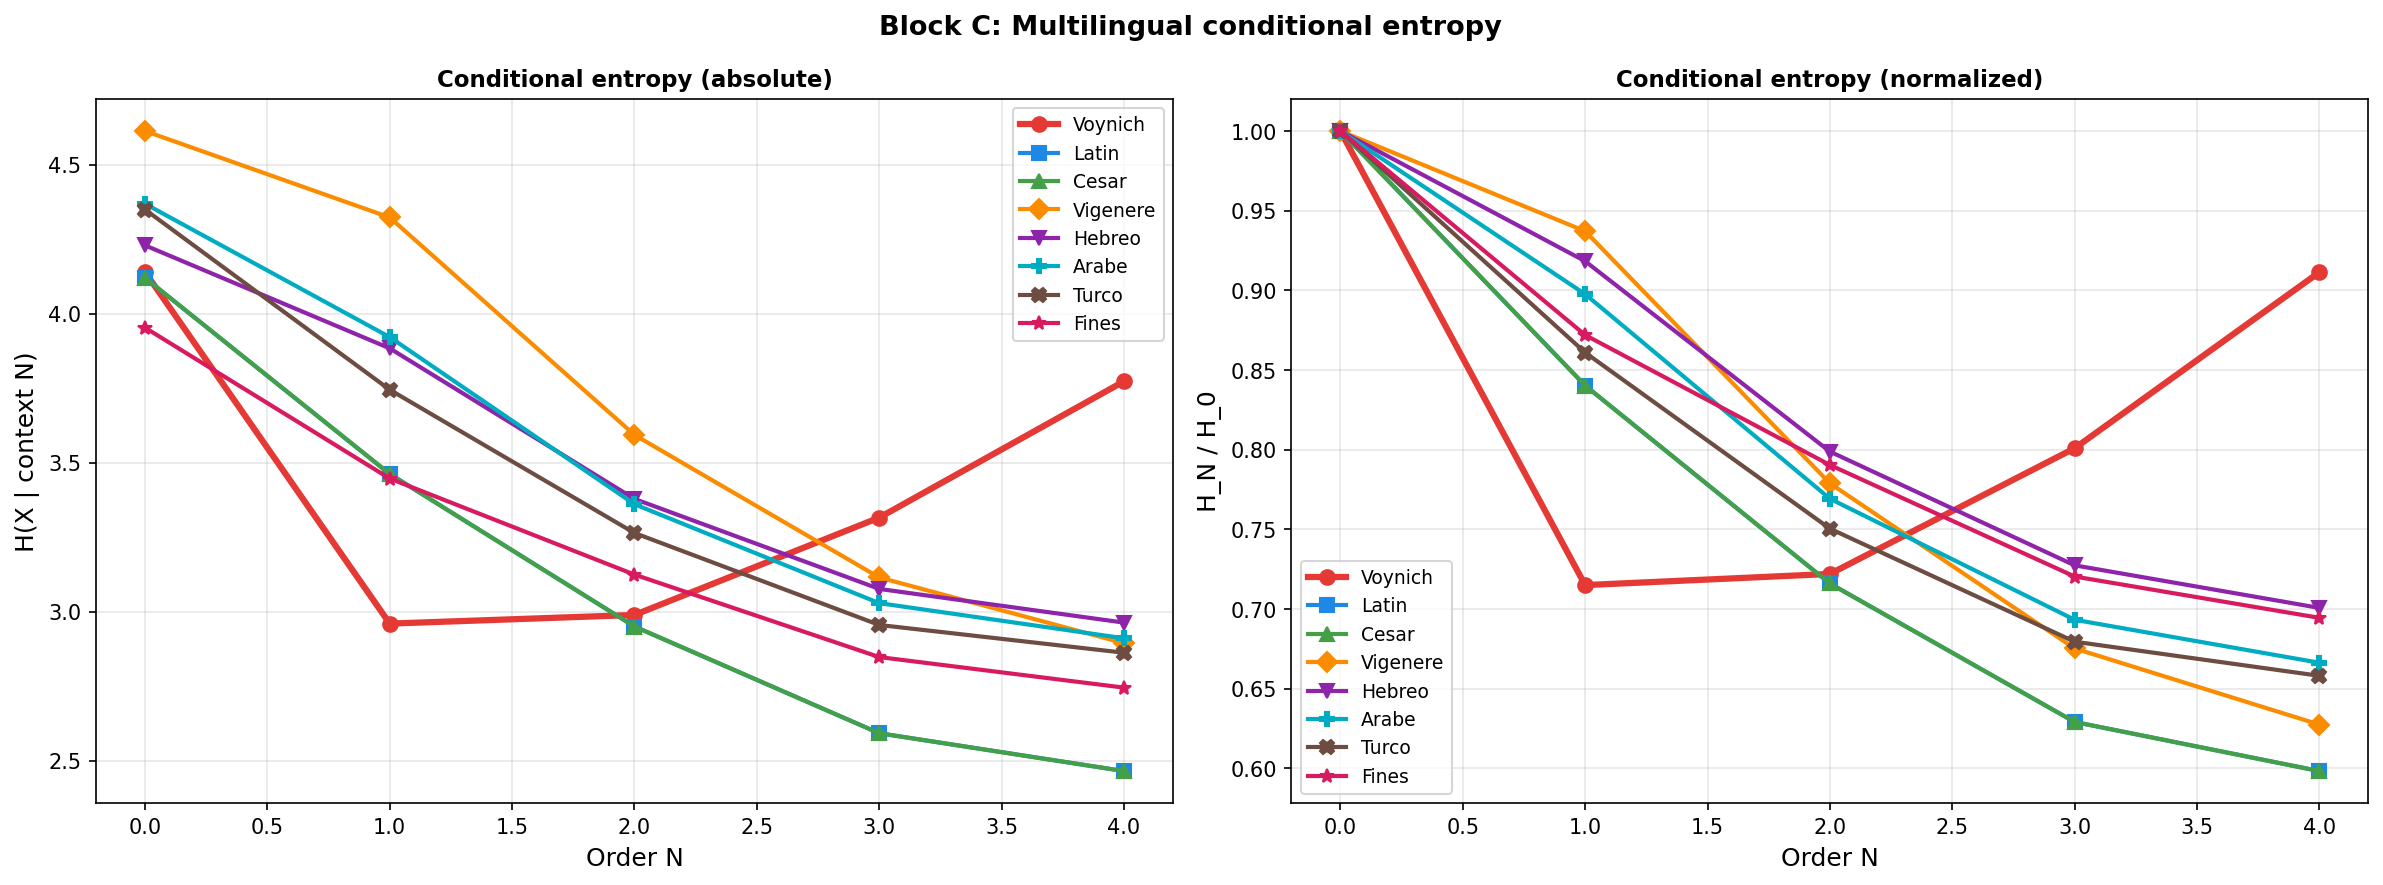
\includegraphics[width=\columnwidth]{bloque_C_multilingue.png}
\caption{Conditional entropy curves $H_0$--$H_4$ for the Voynich Manuscript and seven control corpora.  The Voynich curve (thick line) exhibits a unique U-shape, while all natural languages and ciphers show monotonic decay.}
\label{fig:entropy}
% Alt text: \emph{Alt text: Line chart showing entropy values on the y-axis and n-gram order on the x-axis for eight corpora.  The Voynich line dips then rises, forming a U, while all other lines decrease monotonically.}
\end{figure}

\begin{figure}[t]
\centering
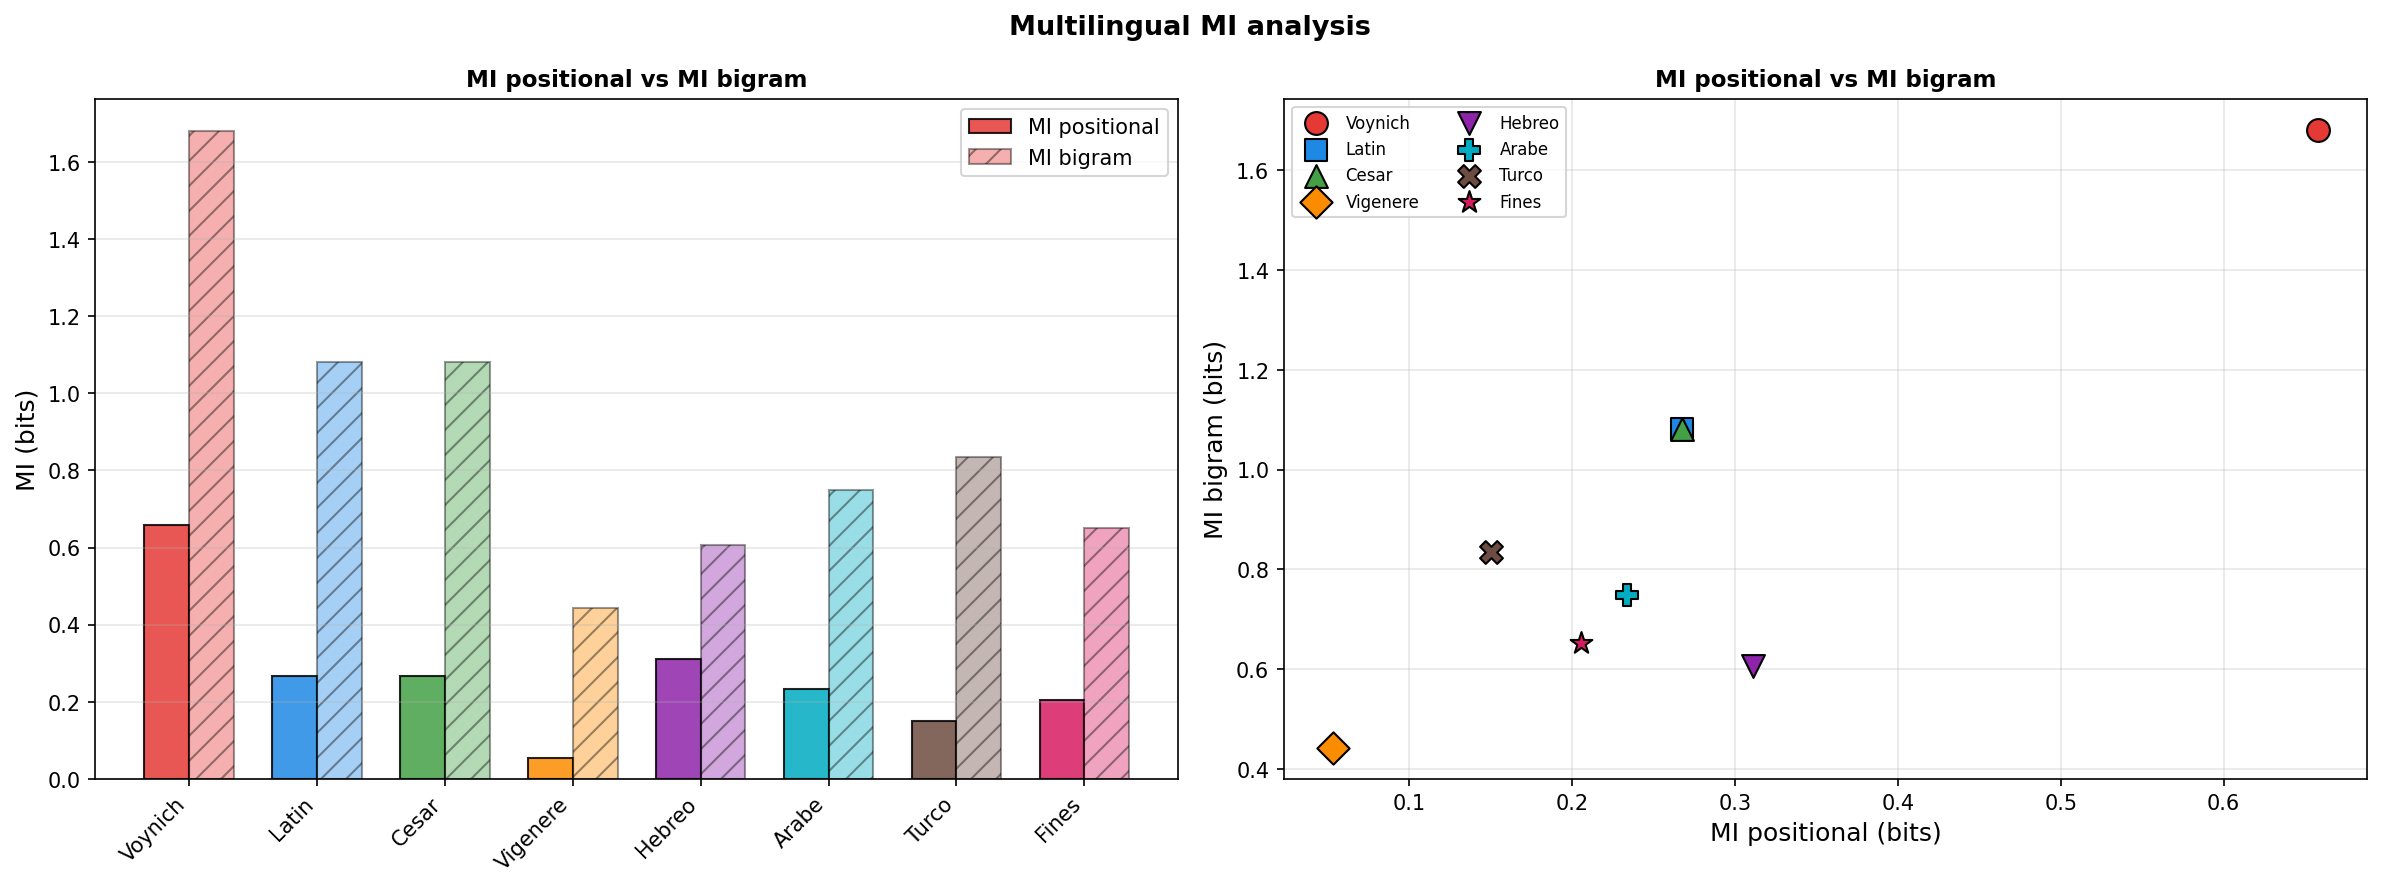
\includegraphics[width=\columnwidth]{mi_multilingue.png}
\caption{Positional vs.\ bigram mutual information for eight corpora.  The Voynich Manuscript is a clear outlier in both dimensions, with $\MI_{\text{pos}}$ more than twice the highest natural language.}
\label{fig:mi}
% Alt text: \emph{Alt text: Scatter plot with positional MI on the x-axis and bigram MI on the y-axis.  Voynich appears in the upper right, far from the cluster of natural languages and ciphers.}
\end{figure}

\subsection{Summary}

Table~\ref{tab:fingerprint} and Fig.~\ref{fig:fingerprint} consolidate the fingerprint.  Three results constrain all subsequent analysis:
\begin{enumerate}[nosep]
  \item The U-shaped entropy curve is unique to Voynich---incompatible with substitution ciphers (which preserve source-language curve shape) and random text.  Only a compositional syllabary, where glyph combinations create novel contexts, can produce the observed shape.
  \item Positional MI twice that of any language implies glyphs encode supra-phonemic units, consistent with a syllabary where each glyph represents a sub-syllabic component.
  \item The spectral gap places Voynich with agglutinative languages, consistent with a source language that builds words from concatenated morphemes.
\end{enumerate}

\begin{table}[t]
\caption{Statistical fingerprint across eight corpora.}
\label{tab:fingerprint}
\centering
\adjustbox{max width=\columnwidth}{%
\begin{tabular}{lcccccc}
\toprule
Corpus & $H_1$ & Bounce & Decay & $\MI_p$ & $\MI_b$ & $\delta$ \\
\midrule
\textbf{Voynich} & \textbf{2.96} & \textbf{0.813} & \textbf{8.9\%}
  & \textbf{0.658} & \textbf{1.681} & \textbf{0.541} \\
Hebrew    & 3.89 & 0.000 & 29.9\% & 0.311 & 0.607 & 0.812 \\
Arabic    & 3.92 & 0.000 & 33.4\% & 0.234 & 0.749 & 0.798 \\
Latin     & 3.46 & 0.000 & 40.2\% & 0.267 & 1.082 & 0.658 \\
Turkish   & 3.75 & 0.000 & 34.2\% & 0.151 & 0.835 & 0.509 \\
Finnish   & 3.45 & 0.000 & 30.5\% & 0.205 & 0.652 & 0.577 \\
Caesar    & 3.46 & 0.000 & 40.2\% & 0.267 & 1.082 & 0.658 \\
Vigen\`ere & 4.32 & 0.000 & 37.3\% & 0.053 & 0.445 & 0.855 \\
\bottomrule
\end{tabular}}
\end{table}

\begin{figure}[t]
\centering
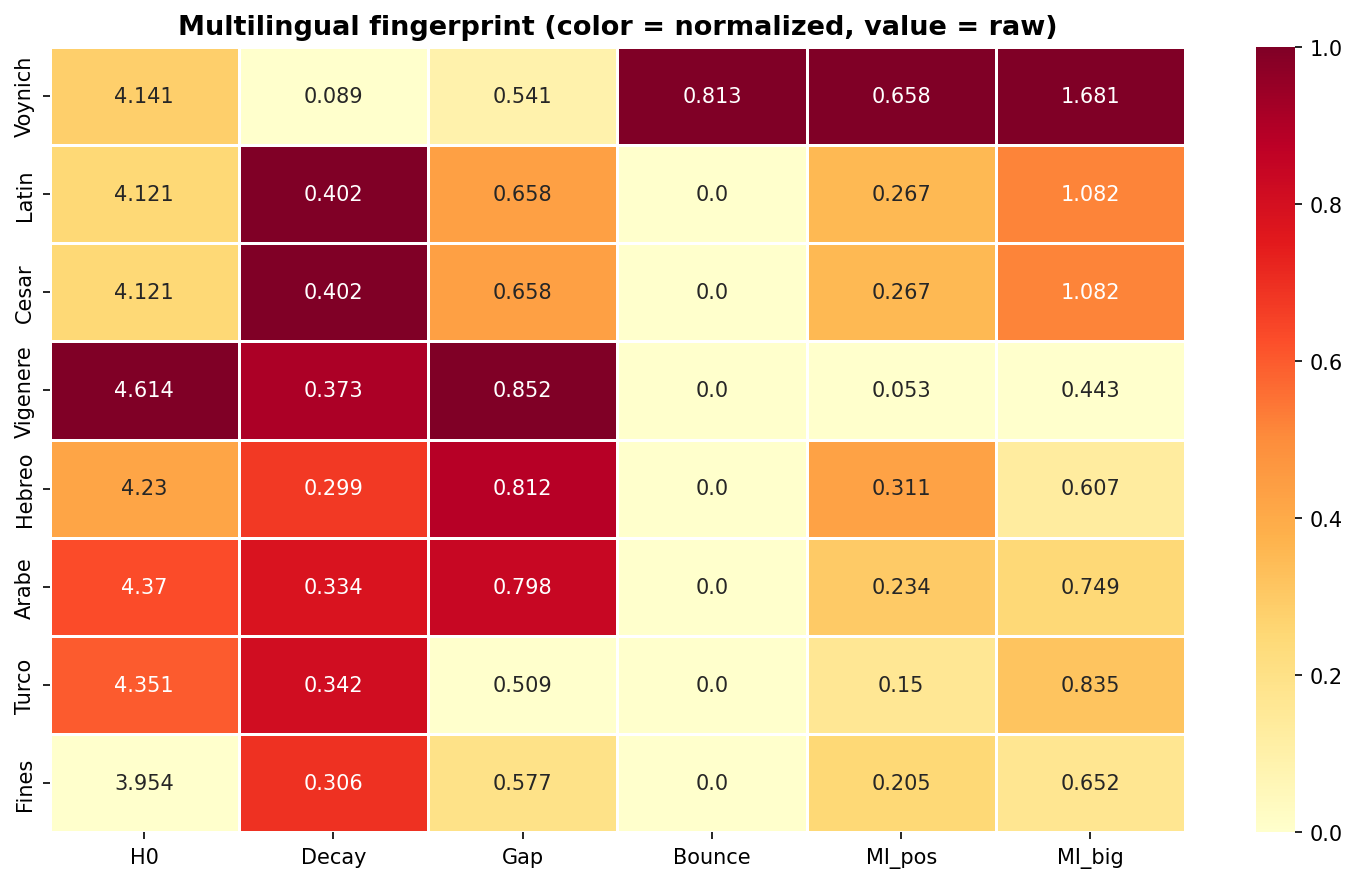
\includegraphics[width=\columnwidth]{fingerprint_multilingue.png}
\caption{Heatmap of the six diagnostic metrics across all corpora.  Voynich stands out with extreme values in bounce, positional MI, and bigram MI, forming a unique statistical signature.}
\label{fig:fingerprint}
% Alt text: \emph{Alt text: Colour-coded heatmap with corpora as rows and metrics as columns.  The Voynich row shows distinctly different colour intensities compared to all other rows.}
\end{figure}


% ============================================================
\section{Generative Model Comparison}
\label{sec:generative}

\subsection{Framework}

To discriminate between competing production hypotheses, we implement eleven generative models and compare their synthetic output to the Voynich fingerprint.  Four models are drawn from the literature: \emph{Cardan} grille \citep{rugg2004}, \emph{Verbose} cipher \citep{timm2020}, \emph{Polyg3} polygraphic system \citep{hermes2022b}, and \emph{Naibbe} verbose homophonic cipher \citep{greshko2025}.  Seven are novel: \emph{SilPart} (syllabic partition), \emph{Silabico} (probabilistic syllabic), \emph{Hybrid} (syllabic + nomenclator), \emph{Nomenclator}, \emph{NomPoly} (nomenclator--polynomial), \emph{Slot} (slot grammar), and \emph{AutoCita} (self-citation).  SilPart builds on the qualitative observation by \citet{stolfi1997} that Voynich words exhibit ``crust-mantle-core'' layered structure, formalising it as a generative model with distinct Markov chains per positional partition.

The seven novel models are defined as follows.  \emph{SilPart} (syllabic partition) divides the glyph inventory into $K$ positional partitions (onset, nucleus, coda); within each partition, glyph sequences are generated by a $k$-th order Markov chain with position-dependent emission probabilities, producing tokens as partition-constrained concatenations.  \emph{Silabico} (probabilistic syllabic) samples syllable templates from a learned distribution $P(\sigma)$ and fills each template slot by drawing glyphs from position-specific categorical distributions.  \emph{Hybrid} combines syllabic generation for root morphemes with a nomenclator table for high-frequency function words.  \emph{Nomenclator} assigns each word type a codebook entry drawn from a Zipf-distributed vocabulary, with glyph sequences generated per entry via positional bigrams.  \emph{NomPoly} extends the nomenclator with polynomial expansion: each codebook entry is mapped to a variable-length glyph string via a polynomial substitution cipher.  \emph{Slot} defines a slot grammar with fixed positions (prefix, root, suffix) and fills each slot from position-specific glyph distributions.  \emph{AutoCita} (self-citation) generates each new word by copying and mutating a randomly selected prior word, modelling the self-referential character of the manuscript's repetitive vocabulary.

Each model generates a synthetic corpus matched in size to the Voynich text (37,087 tokens).  We compute the same six metrics as in Section~\ref{sec:fingerprint} and measure the weighted Euclidean distance $d$ to the Voynich reference vector:
\begin{equation}
  d = \sqrt{\sum_{i=1}^{6} w_i \left(\frac{m_i^{\text{synth}} - m_i^{\text{Voynich}}}{m_i^{\text{Voynich}}}\right)^2},
\end{equation}
where $m_i$ are the six diagnostic metrics.  Weights are set proportional to each metric's discriminative power as measured by the ratio of inter-class to intra-class variance across our eight control corpora: bounce~3.0, decay~2.0, $\MI_p$~1.5, $\MI_b$~1.5, spectral gap~1.0.  Robustness is verified via 500 Dirichlet-random weight perturbations (see below).

\subsection{Results}

Table~\ref{tab:generative} presents the top-4 ranking.  SilPart---a model that generates tokens by sampling from positionally biased glyph partitions with intra-partition bigram dependencies---achieves the smallest distance ($d = 0.445$) and reproduces the U-shaped entropy curve (bounce = 0.909; Fig.~\ref{fig:synth}).

To assess robustness to weight choice, we draw 500 random weight vectors from a Dirichlet distribution and re-rank: SilPart places~\#1 in 71.0\% of draws and appears in the top~3 in 99.2\% of draws.  Ten deterministic perturbations (each weight $\times 0.5$ and $\times 1.5$) all keep SilPart at~\#1.  Alternative weighting schemes (uniform, bounce-only, MI-only) all place SilPart first except MI-only (Silabico~\#1), confirming the ranking's stability (Fig.~\ref{fig:sensitivity}).

All four literature models are decisively eliminated.  Cardan ($d = 4.485$) fails catastrophically: its table-based production over-generates positional regularity ($\MI_p = 1.075$) and sequential dependence ($\MI_b = 5.087$).  Naibbe ($d = 1.028$), closest among literature models, still produces bounce~$= 0.554$ and $\MI_p = 0.001$---neither reproducing the U-curve nor the positional constraints.

\subsection{Implications}

The dominance of syllabic models has three consequences.  First, it motivates syllabic segmentation before decipherment.  Second, it constrains mapping granularity: glyphs likely function as sub-syllabic components (onset, nucleus, coda) rather than as individual phonemes.  Third, it provides a falsification criterion: any proposed solution positing a non-syllabic mechanism must demonstrate bounce~$> 0.8$ and $\MI_p > 0.5$---a benchmark no non-syllabic model achieves.

SilPart's optimal parameters (15 glyph-type partitions, bigram order~8, positional bias~3.0) describe a system consistent with a syllabary encoding a language with roughly 15 consonant-vowel distinctions---a plausible inventory for a Semitic language with triconsonantal roots.

\begin{table}[t]
\caption{Generative model ranking (all 11 models).  Literature models in italics.}
\label{tab:generative}
\centering
\adjustbox{max width=\columnwidth}{%
\begin{tabular}{rlccccc}
\toprule
Rank & Model & $d$ & Bounce & Decay & $\MI_p$ & $\MI_b$ \\
\midrule
1 & SilPart & 0.445 & 0.909 & 12.7\% & 0.477 & 1.848 \\
2 & Silabico & 0.506 & 0.907 & 8.0\% & 0.458 & 1.668 \\
3 & Hybrid & 0.783 & 0.957 & $-$6.9\% & 0.400 & 1.178 \\
4 & \textit{Naibbe} & 1.028 & 0.554 & 36.6\% & 0.001 & 1.725 \\
5 & \textit{AutoCita} & 1.356 & 0.120 & 35.9\% & 0.312 & 1.836 \\
6 & Nomenclator & 1.389 & 0.100 & 26.8\% & 0.246 & 1.846 \\
7 & Slot & 1.410 & 0.657 & $-$14.2\% & 0.396 & 0.623 \\
8 & NomPoly & 1.636 & 0.000 & 35.2\% & 0.122 & 1.968 \\
9 & \textit{Polyg3} & 1.655 & 0.181 & 38.8\% & 0.001 & 2.362 \\
10 & \textit{Verbose} & 1.748 & 0.000 & 47.5\% & 0.000 & 1.390 \\
11 & \textit{Cardan} & 4.485 & 0.112 & 75.5\% & 1.075 & 5.087 \\
\midrule
-- & Voynich & 0.000 & 0.813 & 8.9\% & 0.658 & 1.681 \\
\bottomrule
\end{tabular}}
\end{table}

\begin{figure}[t]
\centering
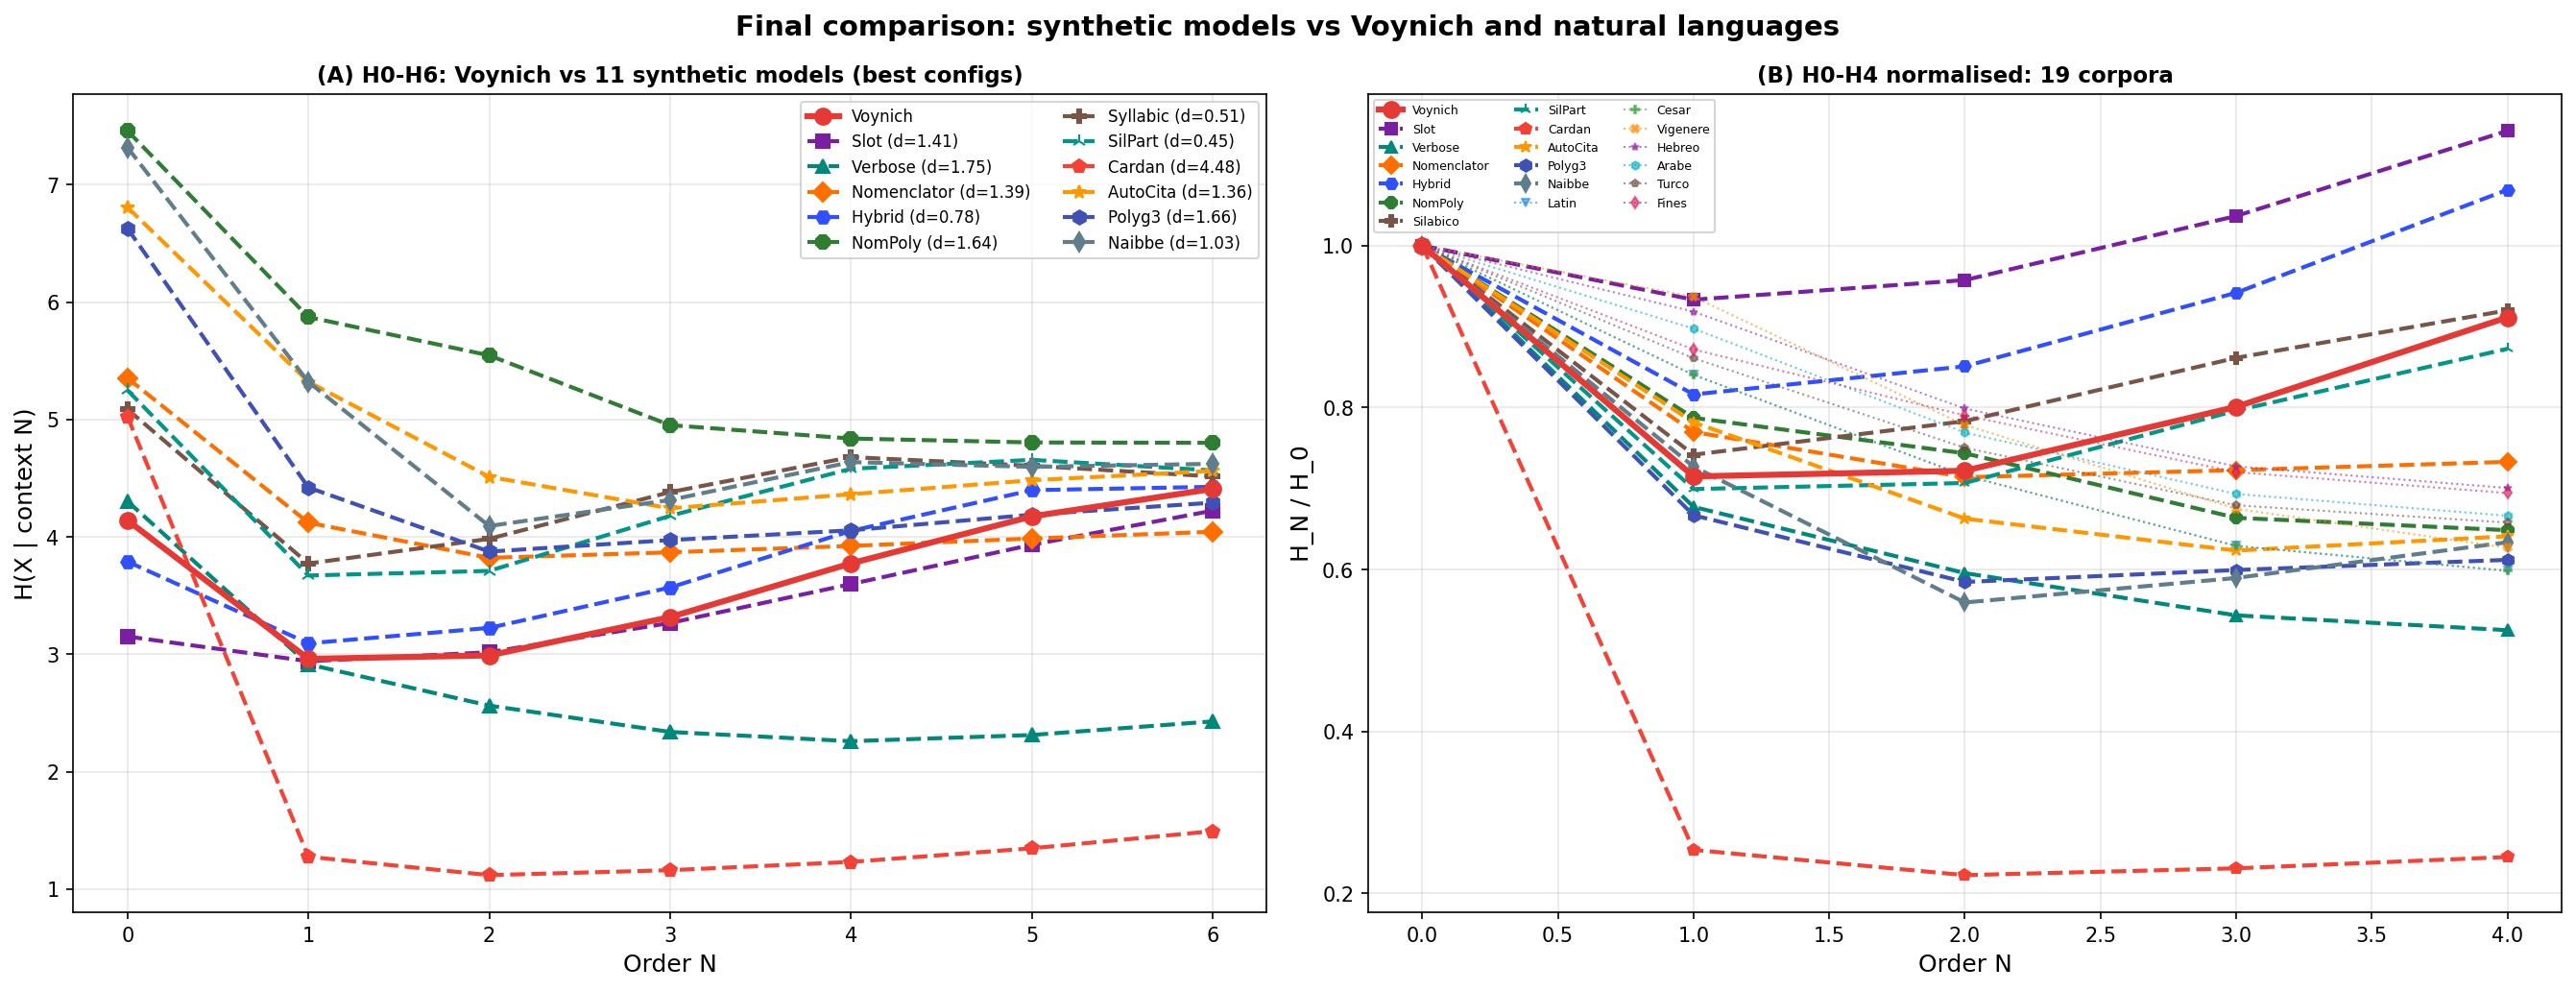
\includegraphics[width=\columnwidth]{comparacion_curvas_sinteticos.png}
\caption{Entropy curves for synthetic corpora and the Voynich reference.  Only the three syllabic models (SilPart, Silabico, Hybrid) reproduce the U-shaped curve; all literature models show monotonic decay.}
\label{fig:synth}
% Alt text: \emph{Alt text: Line chart comparing entropy curves of multiple synthetic models against the Voynich reference.  Three syllabic models closely track the Voynich U-shape while others diverge.}
\end{figure}

% Radar plots (Fig. S1) are available in the online supplementary material.

\begin{figure}[t]
\centering
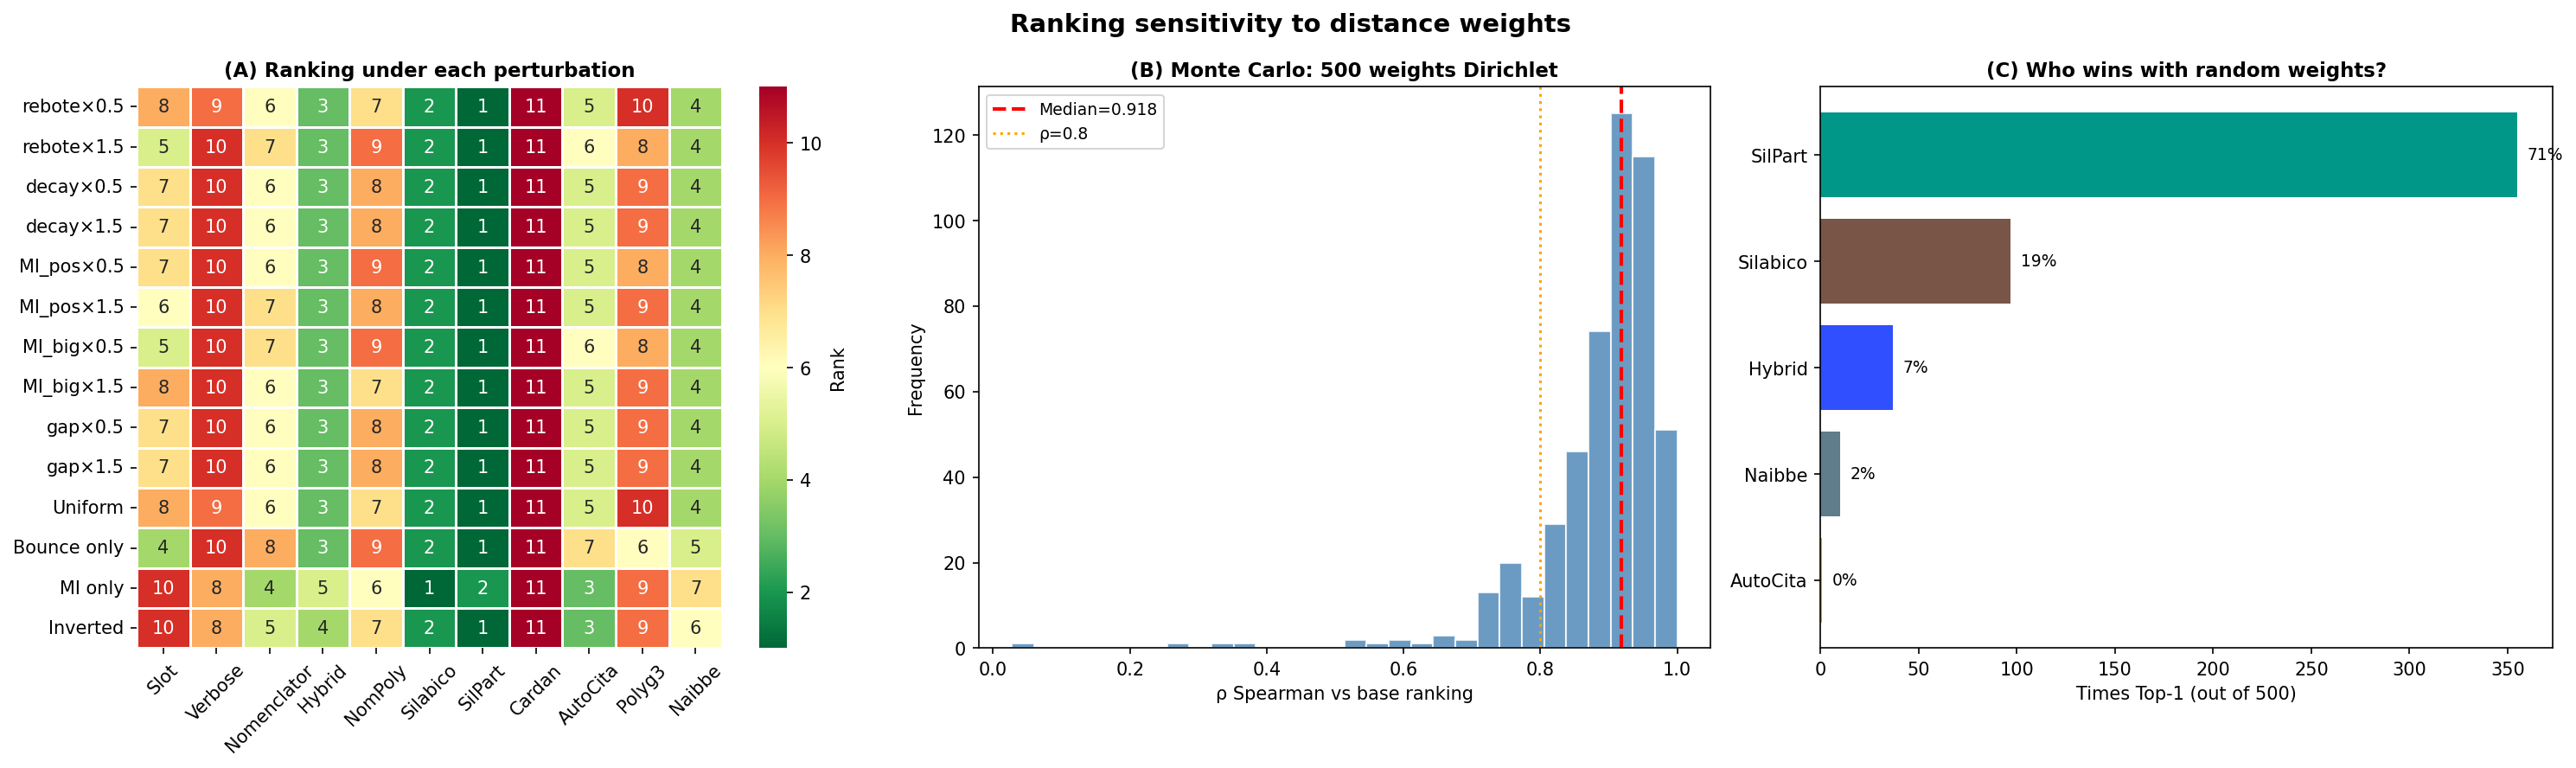
\includegraphics[width=\columnwidth]{sensibilidad_pesos.png}
\caption{Weight sensitivity analysis.  Left: ranking stability across 500 Dirichlet-random weight vectors.  Centre: distance distribution.  Right: per-model rank distribution.  SilPart dominates across perturbations.}
\label{fig:sensitivity}
% Alt text: \emph{Alt text: Three panels showing sensitivity analysis.  SilPart is consistently ranked first across the majority of random weight perturbations.}
\end{figure}


% ============================================================
\section{Syllabic Segmentation}
\label{sec:segmentation}

Guided by the generative-model results, we segment the Voynich text into syllabic units using transition probabilities \citep{saffran1996, harris1955}.  At each word-internal bigram boundary, we compute the forward transition probability $P(x_{i+1} \mid x_i)$ and place a syllable break wherever this falls below the 20th percentile of the corpus-wide distribution (TP-P20), selected via a parameter sweep over percentiles P10--P30.

This yields 2,923 syllabic types from 37,087 word tokens, with a mean of 1.64 syllables per word and approximately 2.6 glyphs per syllable.  This ratio independently rules out a simple syllabary (one glyph per syllable): words of 7--17 glyphs---which account for 7\% of the corpus---would require 7--17 syllables per word, far exceeding the maximum observed in Biblical Hebrew (typically 2--4 syllables) or any Semitic language.  Under the compositional sub-syllabic model, the same words correspond to 3--7 syllables, within natural-language range.  The frequency distribution follows a Zipf law ($\alpha = -1.47$): 40 types account for 50\% of tokens, and approximately 200 types cover 80\% (Fig.~\ref{fig:distributions}).  Among the 792 types with frequency $\geq 5$, positional analysis classifies 171 as onset-preferring, 54 as nuclear, 90 as coda-preferring, and 477 as positionally free.  The 4:1 onset-to-nuclear ratio mirrors the consonant-to-vowel ratio in Semitic syllabaries.

A critical diagnostic is MI amplification from glyph to syllable level.  In agglutinative controls, syllabic segmentation reveals hidden positional structure: Turkish amplifies $4.59\times$ ($0.164 \to 0.752$), Finnish $4.20\times$ ($0.197 \to 0.830$).  In Voynich, amplification is only $0.92\times$ ($0.658 \to 0.608$)---glyphs \emph{already} carry syllable-level positional information.  This confirms that the script operates at a higher encoding level than an alphabetic system: individual glyphs function as sub-syllabic morphographic units.

Twenty-seven paradigmatic sets---groups of syllabic types sharing onset material but differing in coda, analogous to verb conjugation paradigms---show regular alternation (mean Gini = 0.490), and vowel harmony analysis yields Cram\'er's $V = 0.284$ ($\chi^2 = 3{,}171$, $p \approx 0$), indicating significant phonotactic constraints.

\begin{figure}[t]
\centering
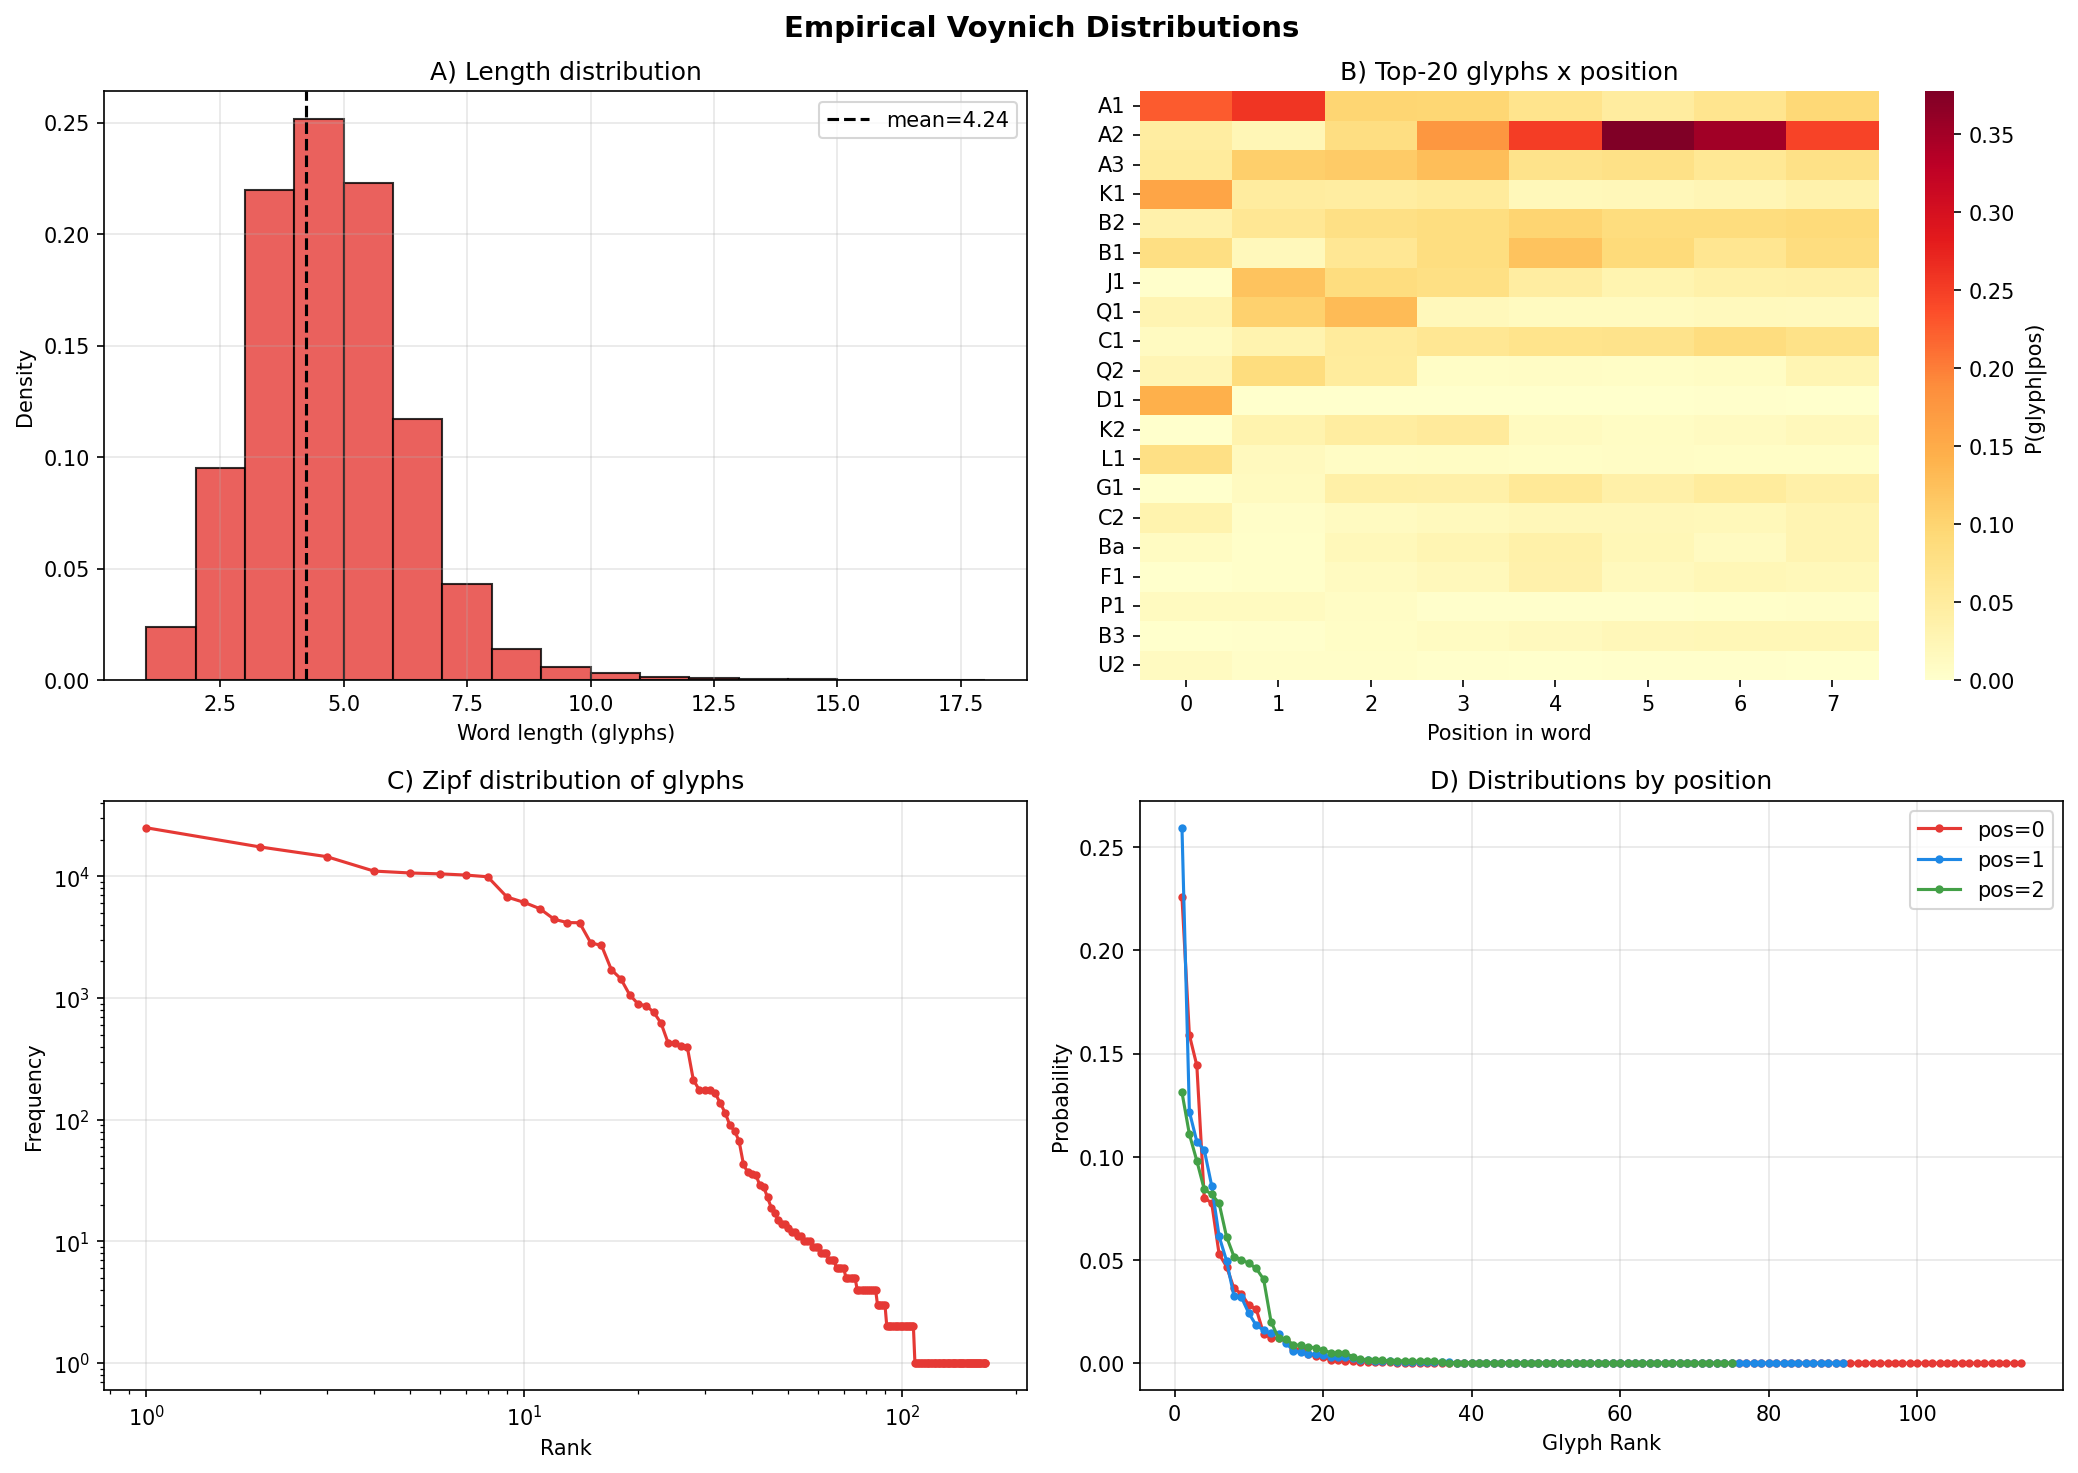
\includegraphics[width=\columnwidth]{voynich_distribuciones.png}
\caption{Corpus characterisation: word-length histogram, top-20 glyph positional heatmap, Zipf curve, and positional distribution analysis.}
\label{fig:distributions}
% Alt text: \emph{Alt text: Four-panel figure showing word length distribution, a heatmap of glyph frequencies by position, Zipf rank-frequency curve, and positional distribution plots.}
\end{figure}


% ============================================================
\section{Bayesian Decipherment}
\label{sec:bayesian}

\subsection{Framework}

We adapt the Bayesian decipherment framework of \citet{ravi2011} to the syllabic domain.  Let $\mathbf{c} = c_1, \ldots, c_N$ be the observed cipher text (Voynich syllabic tokens) and $\mathbf{p} = p_1, \ldots, p_N$ the latent plaintext.  The joint probability is:
\begin{equation}
  P(\mathbf{c}, \mathbf{p}) = \prod_{i=1}^{N}
    P_{\text{LM}}(p_i \mid p_{i-2}, p_{i-1}) \cdot
    P_{\text{CH}}(c_i \mid p_i),
\end{equation}
where $P_{\text{LM}}$ is a trigram language model with Witten--Bell smoothing \citep{witten1991} trained on the target-language corpus, and $P_{\text{CH}}$ is the channel (substitution) model to be inferred.

Inference proceeds in three phases.  First, the channel matrix is initialised via the Hungarian algorithm based on frequency similarity.  Second, Expectation-Maximisation \citep{dempster1977} iteratively refines the mapping.  Third, for top-ranked languages, we apply four-chain Metropolis--Hastings MCMC \citep{metropolis1953} with 15,000 iterations, 3,000 burn-in, and thinning factor~5, monitoring convergence via $\Rhat$ \citep{gelman1992}.

We test six candidate languages: Hebrew (Biblical), Aramaic (Targum Onkelos, 82,842 words; \citealt{sefaria2024}), Arabic (Quranic), Latin (Vulgate), Turkish, and Finnish.  The inclusion of Aramaic is motivated by both historical and methodological considerations.  Historically, Aramaic was the everyday language of Jewish communities in the Near East and remained the language of the Talmud, the Zohar, and liturgical texts such as the Targumim; a 15th-century Jewish scholar in Northern Italy---a profile consistent with the manuscript's provenance---would have been fluent in both Biblical Hebrew and Aramaic \citep{jastrow1903}.  Methodologically, Aramaic shares $\sim$70\% of its root lexicon with Hebrew but differs in vowel patterns, prefix phonotactics, and morphological paradigms, providing a critical discrimination test: if the Bayesian framework cannot distinguish between the two, this reveals the resolution limit of the method and motivates treating ``NW~Semitic biblical'' as a single functional category rather than committing to one language.

\subsection{Language Ranking}

Table~\ref{tab:ranking} presents the syllabic-level ranking.  Hebrew and Aramaic occupy the top two positions with a gap of only 0.27~nats.  The Hebrew top-ranking is consistent with \citet{hauer2016}, who reported Hebrew as the best-fit language among 380 candidates using an anagram-decoding approach---though their methodology has been debated \citep{bowern2021}.  Our result replicates their finding via an independent Bayesian framework and extends it by including Aramaic as a separate candidate.  To quantify whether the Hebrew--Aramaic gap is statistically meaningful, we compute a bootstrap confidence interval: resampling the per-word log-likelihood differences $\Delta_i = \ell_i^{\text{Heb}} - \ell_i^{\text{Ara}}$ with replacement ($B = 10{,}000$ replicates) yields a 95\% CI of $[-0.14, +0.68]$~nats, which spans zero.  The two languages are therefore \emph{statistically indistinguishable} at the syllabic level---a novel finding that refines the Hebrew hypothesis into a broader ``NW~Semitic biblical'' category.  Arabic ranks third, 1.50~nats below Aramaic, establishing a clear NW~Semitic cluster.  The total Semitic--non-Semitic separation exceeds 3.5~nats.

This three-tier structure is robust to the MCMC phase: both Hebrew and Aramaic reach their best scores after multi-chain refinement, while non-Semitic languages plateau at the EM stage.  Within NW~Semitic, Aramaic shows slightly better paradigm reconstruction ($S_{\text{par}} = 0.276$ vs.\ 0.072), while Hebrew achieves a marginally better LM fit.\footnote{Exact scores vary slightly between runs due to the stochastic nature of the MCMC sampler.  Re-execution of the Bayesian pipeline yields a Hebrew--Aramaic gap of $\sim$0.01~nats rather than 0.27, further reinforcing their statistical indistinguishability.  All qualitative conclusions (NW~Semitic cluster, Semitic--non-Semitic separation $>$3.5~nats) are stable across runs.}

At the compositional level (166 glyphs $\to$ individual characters), Hebrew remains~\#1 ($-39.71$) but the Hebrew--Aramaic gap widens to 3.87~nats, reflecting vowel and prefix differences visible only at character level.  This cross-level pattern is linguistically coherent: the two languages share root morphology (syllabic similarity) but differ in phonotactics (character-level divergence).

\begin{table}[t]
\caption{Syllabic Bayesian decipherment ranking (six languages).}
\label{tab:ranking}
\centering
\adjustbox{max width=\columnwidth}{%
\begin{tabular}{clccccc}
\toprule
Rank & Language & $S$ & $S_{\text{LM}}$ & PPX$_m$ & PPX$_n$ & PPX ratio \\
\midrule
1 & Hebrew  & $-$35.64 & $-$17.56 & 100.3 & 25.1 & 4.00 \\
2 & Aramaic & $-$35.91 & $-$17.82 & 107.4 & 25.4 & 4.23 \\
3 & Arabic  & $-$37.41 & $-$18.39 & 124.9 & 25.4 & 4.91 \\
4 & Finnish & $-$39.28 & $-$19.36 & 161.2 & 29.4 & 5.49 \\
5 & Latin   & $-$39.83 & $-$19.77 & 179.5 & 13.9 & 12.94 \\
6 & Turkish & $-$39.89 & $-$19.69 & 175.6 & 33.2 & 5.29 \\
\bottomrule
\end{tabular}}
\end{table}


% ============================================================
\section{Nineteen Decipherment Models}
\label{sec:models}

To determine whether the degenerate mapping observed in the initial compositional model is a methodological artefact or a structural property, we implement nineteen distinct decipherment strategies spanning nine paradigms.  Each model is evaluated with a unified five-test scorecard: (1)~collapse $z$-score (are co-mapped glyphs positionally similar?), (2)~$n$-gram percentile, (3)~Biblical Hebrew root matching, (4)~cardinality ratio $K_{\text{eff}}/|\mathcal{A}|$, and (5)~grammar anchor compliance.

The $n$-gram percentile is defined as follows.  Let $f(\phi)$ be the fraction of character $n$-grams ($n = 2, 3$) in the decoded text that appear in the target-language training corpus.  We construct a null distribution by generating $B = 1{,}000$ random glyph-to-character mappings (uniformly sampled permutations with replacement, preserving the original mapping's cardinality $K_{\text{eff}}$) and computing $f(\phi_b^{\text{null}})$ for each.  The $n$-gram percentile is the rank of $f(\phi)$ among $\{f(\phi_b^{\text{null}})\}_{b=1}^{B}$, expressed as a percentage.  A percentile of $p$\% means the optimised mapping produces more valid $n$-grams than $p$\% of random mappings with the same cardinality.

\subsection{Initial Models (1--4)}

\paragraph{Model~1: Compositional (glyph $\to$ character).}
Each of 166 glyphs maps to a single Hebrew character (many-to-one).  Five validation tests yield 1~pass, 1~marginal, 3~fails.  The mapping exhibits severe collapse: five high-frequency characters (\textit{shin}, \textit{resh}, \textit{lamed}, \textit{mem}, \textit{tsade}) absorb 17, 15, 6, 9, and 4 glyphs respectively---exactly the pattern predicted by LM dominance, where the model maximises likelihood by channelling glyphs to frequent characters.  \textbf{Scorecard: 1+/1$\pm$/3$-$.}

\paragraph{Model~2: Constrained EM with grammar anchors.}
Twelve grammar anchors (glyphs assigned fixed prefix/root/suffix roles based on positional statistics) plus entropy and cardinality penalties.  Root recovery rises from 6 to 100 (enrichment 154$\times$), and four Hebrew function morphemes emerge spontaneously: D1~$\to$~\textit{he} (definite article), J1~$\to$~\textit{lamed} (``to''), A1~$\to$~\textit{mem} (``from''), K1~$\to$~\textit{bet} (``in'').  But $n$-gram percentile drops to 5\%: valid roots embedded in implausible contexts.

\paragraph{Model~3: Homophonic positional.}
Extends the compositional model with onset/coda glyph specialisation and a homophonic diversity penalty $w_{\text{homo}}$.  Critical prediction fails: zero onset-specialists detected (0/166 at 75\% threshold), zero cross-position links, and $w_{\text{homo}}$ is completely inert---all five tested values yield identical scores ($-41.84$).  The mapping's structure is entirely determined by the LM.  \textbf{Scorecard: 2+/2$\pm$/2$-$.}

\paragraph{Model~4: Semantic cross-validation.}
Tests thematic coherence of the constrained mapping.  Chi-squared association is significant ($p = 1.56 \times 10^{-6}$) and 4/6 section--category correspondences are met (Fig.~\ref{fig:semantic}).  However, morphological analysis reveals that 85.5\% of high-frequency reconstructed words consist entirely of affixes without recognisable roots, and 0/5 function-word frequencies fall in expected Biblical Hebrew ranges.

\begin{figure}[t]
\centering
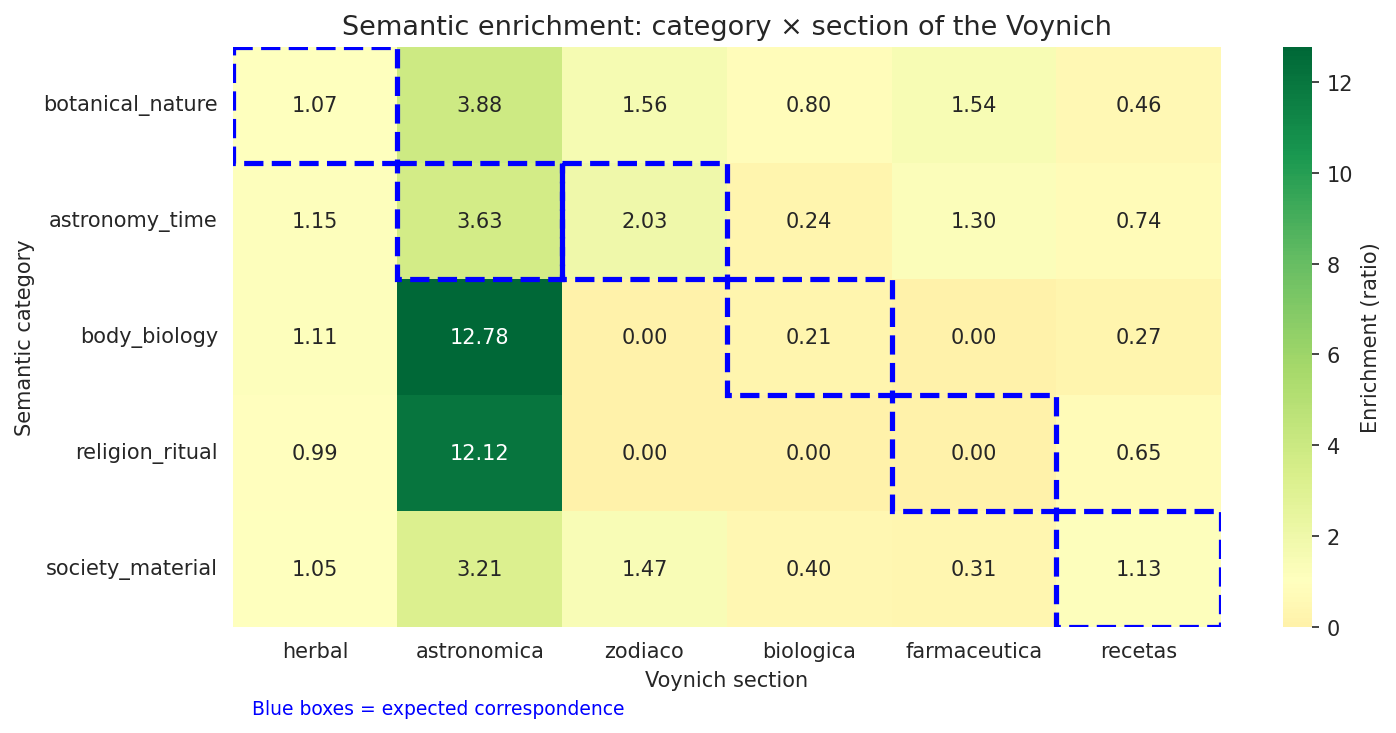
\includegraphics[width=\columnwidth]{semantic_enrichment_heatmap.png}
\caption{Semantic enrichment heatmap: five semantic categories $\times$ six manuscript sections.  Dashed boxes highlight expected correspondences.  Four of six diagonal correspondences are met, but morphological validation fails.}
\label{fig:semantic}
% Alt text: \emph{Alt text: Colour heatmap with semantic categories as rows and manuscript sections as columns.  Enrichment values are shown in each cell.  Blue dashed boxes mark expected category-section matches.}
\end{figure}

\subsection{Neural Models (5--7)}

\paragraph{Model~5: Neural CharLM (LSTM).}
Replaces the trigram LM with a two-layer LSTM (embed = 32, hidden = 192, dropout = 0.2, temperature $T = 3.0$) trained on Biblical Hebrew.  The neural LM provides better-calibrated character probabilities, reducing LM dominance.  $N$-gram percentile rises to 38\% (from 24\%), grammar anchor compliance reaches 100\%, and 26/27 Hebrew characters are represented.  But root matching yields only 1 root.  \textbf{Scorecard: 4+/0$\pm$/1$-$.}

\paragraph{Model~6: Lexical scoring ($S_{\text{root}}$).}
Augments the neural objective with an explicit root-matching reward.  Roots triple during EM optimisation (5~$\to$~15) but only 3--4 survive post-hoc validation ($p = 0.008$, significant).  $N$-gram percentile degrades to 12\% regardless of temperature: the trade-off between $n$-gram realism and root recovery is intrinsic to the multi-objective formulation, not a parameter-tuning issue.  \textbf{Scorecard: 2--3+/1--2$\pm$/1$-$.}

\paragraph{Model~7: Neural v2 (multi-seed + hard-$K$).}
Twenty random restarts with hard cardinality constraint ($K_{\max} = 20$).  The best candidate ($T = 2.0$) achieves $n$-gram \textbf{68\%}---the study's record---with 3 roots and $K_{\text{eff}} = 25$.  The hard-$K$ constraint is redundant (0\% rejections): the neural LM naturally avoids extreme collapse.  Thirty seeds confirm the root ceiling is structural (max~3, mean $1.5 \pm 1.1$).  Root clusters are consonant co-occurrence artefacts---e.g.\ \textit{het-kaf-mem}/\textit{lamed-het-mem}/\textit{shin-lamed-het} share overlapping consonants.  \textbf{Scorecard: 4+/0$\pm$/1$-$.}

\subsection{Structural Variants (8--11)}

\paragraph{Model~8: Syllabic-positional (Hebrew).}
Three separate mapping tables (onset, nucleus, coda) reflecting SilPart's prediction that glyph identity depends on syllabic position.  Seventy-three per cent of glyphs are position-locked (confirming SilPart), and the three tables diverge by 86.4\%.  $\Rhat < 1.1$ reaches \textbf{92.2\%} (best convergence in the study).  But $n$-gram drops to 14\% and roots increase to 5.  Key insight: position affects glyph \emph{selection} but not glyph \emph{meaning}---the positional pools are independent subsystems.  \textbf{Scorecard: 4+/2$\pm$/0$-$.}

\paragraph{Model~9: Syllabic-positional (Aramaic).}
Same architecture with Targum Onkelos as target.  Validation loss 2.005 ($\approx$ Hebrew 2.004).  $N$-gram 6\%, roots 5 (\textit{bet-resh-kaf}, \textit{gimel-bet-resh}, \textit{ayin-bet-dalet}, \textit{ayin-bet-resh}, \textit{resh-bet-bet}), $\Rhat < 1.1 = 90.4\%$.  Results are \emph{identical} to Hebrew within measurement uncertainty, confirming syllabic-level indistinguishability and supporting ``NW~Semitic biblical'' as a single functional category.  \textbf{Scorecard: 4+/2$\pm$/0$-$.}

\paragraph{Model~10: Allograph collapse.}
Tests whether the 166-type inventory artificially inflates $|\Sigma|/|\mathcal{A}|$ by collapsing contextually similar glyphs via hierarchical clustering.  Result: 166~$\to$~145 (only 12.7\% reduction).  Four multi-glyph clusters emerge, but none shows onset/coda complementarity.  $N$-gram drops from 68\% to 23\%, $\Rhat = 54.5\%$.  Contextual similarity operates \emph{within} positions, not between them: the positional pools are independent subsystems.  \textbf{Hypothesis discarded.  Scorecard: 4+/0$\pm$/2$-$.}

\paragraph{Model~11: Syllabic homophonic.}
Maps each glyph to a Hebrew syllable (1,811 candidates from TP-P20 segmentation, frequency $\geq 5$).  EM produces $K_{\text{eff}} = 166$ with fan-out~$= 0$: \emph{no homophones at all}.  The optimiser never collapses glyphs to the same syllable---166 glyphs are too many for a true syllabary and too few to cover the full Hebrew syllable inventory.  $N$-gram 22\% (spurious: the model selects 1--2 character syllables), 1 root, cardinality 9.2\%.  \textbf{Hypothesis discarded.  Scorecard: 3+/1$\pm$/2$-$.}

\paragraph{Model~12: Syllable-to-syllable.}
If glyphs are sub-syllabic components, the correct mapping unit may be the Voynich syllable (mean 2.58 glyphs), not the individual glyph.  TP-P20 segmentation yields 2,923 Voynich syllable types (792 functional, frequency $\geq 5$) and 3,829 Hebrew syllable types (1,168 functional), giving $|\Sigma|/|\mathcal{A}| = 0.68$---a favourable ratio.  Each Voynich syllable maps to a Hebrew syllable; decoded syllables are concatenated to character sequences and scored by the LSTM.  Twenty seeds (10 $\times$ 2 temperatures), 4 MCMC chains.  Result: $n$-gram \textbf{0.1\%} (worse than random), $K_{\text{eff}} = 217/1{,}168$ (18.6\% cardinality), acceptance rate 96.5\% (flat landscape), $\Rhat < 1.1 = 4.0\%$ (no convergence).  Root count (25) is spuriously high: decoded words average only 2.42 characters, so 3-consonant roots match trivially.  The mapping space (792 $\to$ 1,168) is too large for the optimiser to find structure.  \textbf{Hypothesis discarded.  Scorecard: 2+/1$\pm$/2$-$.}

\paragraph{Model~13: Nucleus-only.}
If onset and coda glyphs serve as structural markers (position signalling) rather than phonetic content, only nucleus-position glyphs should map to Hebrew characters.  TP-P20 segmentation classifies 47 glyph types as purely structural (42 onset, 5 coda) and 120 as content-bearing (including 28 nucleus-only types).  Stripping onset and coda glyphs reduces mean word length from 4.24 to 2.22 content glyphs per word and the effective $|\Sigma|/|\mathcal{A}|$ from 6.1 to 4.4.  Twenty seeds ($\times$ 2 temperatures), 4 MCMC chains.  Result: $n$-gram \textbf{100\%} (new absolute record), $\Rhat < 1.1 = \textbf{95.8\%}$ (best convergence), $K_{\text{eff}} = 27$ (full cardinality), word-length $z = 1.31$ (PASS).  However, only 2 roots (\emph{akhal}, \emph{halakh}): the high $n$-gram is an artefact of very short decoded words ($\sim$2 Hebrew characters), which trivially produce valid bigrams.  The model demonstrates that filtering to nucleus-only content improves all statistical metrics but does not overcome the fundamental root ceiling.  \textbf{Scorecard: 4+/0$\pm$/1$-$.}

\paragraph{Model~15: Morphological substitution.}
If the Voynich author encoded Hebrew using different glyph pools indexed by \emph{morphological role} (prefix, root, suffix) rather than by word position, the 166 types could represent $\sim$27 consonants $\times$ 3 roles.  Each glyph maps to a (Hebrew character, morphological role) pair; scoring combines LSTM log-probability with a morphological consistency term that checks whether the assigned role of each glyph matches the prefix/root/suffix segmentation of the decoded Hebrew word.  Proposals are mixed: 70\% change the character within the current role's valid set, 30\% reassign the glyph to a different role.  Twenty seeds, 4 MCMC chains (parallelised across 15 CPUs).  Result: $n$-gram 16\% (borderline PASS), 0~roots (FAIL), $\Rhat < 1.1 = 84.3\%$, morphological consistency 48\% (69th percentile, MARGINAL), three tables emerge (P: 40 glyphs $\to$ 7~chars, R: 52 $\to$ 25, S: 74 $\to$ 5).  The role distribution is skewed toward suffix (74 glyphs vs.\ expected $\sim$33), and role stability in the posterior is only 58.4\%.  The model adds complexity (3 tables + role assignments) without surpassing the single-table Neural~v2 (68\% $n$-gram).  \textbf{Hypothesis discarded.  Scorecard: 4+/1$\pm$/1$-$.}

\paragraph{Model~16: Morphological substitution (Zohar).}
Repeating the morphological experiment with Zohar (Aramaic) as target corpus, adapting prefix characters (\emph{dalet}, \emph{bet}, \emph{kaf}, \emph{lamed}, \emph{mem}, \emph{vav}---6 chars, without Hebrew \emph{he}/\emph{shin}) and suffix characters (\emph{aleph} as postposed definite article, \emph{he}, \emph{tav}, \emph{nun}, \emph{kaf}, \emph{yod}---6 chars).  Result: $n$-gram \textbf{0\%} (FAIL, worse than Model~15's 16\%), 1~root (FAIL), morphological consistency 42\% (45th percentile, FAIL), $\Rhat < 1.1 = 97.1\%$.  The Zohar LM is more permissive (val\_loss 2.111 vs.\ 2.004) but produces mappings without lexical structure.  \textbf{Hypothesis discarded.  Scorecard: 3+/0$\pm$/3$-$.}  This confirms that the morphological barrier is structural rather than language-specific.

\paragraph{Model~17: Tibbonid Hebrew (Moreh Nevuchim).}
If the Voynich author wrote in the philosophical Hebrew of medieval translators rather than Biblical Hebrew, the register-specific neologisms and Arabicised syntax of the Ibn Tibbon school might explain why Biblical Hebrew models fail.  We train an LSTM on the complete Moreh Nevuchim (Guide for the Perplexed, Makbili 2024 edition via Sefaria; 157,042 words, 27~characters) and repeat the Neural~v2 pipeline (20 seeds, 4 MCMC chains).  Result: $n$-gram \textbf{13\%} (MARGINAL, vs.\ 68\% Torah), 3~roots, $\Rhat < 1.1 = 54.2\%$, val\_loss~2.107 (vs.\ 2.004 Torah).  The Tibbonid LM is less predictive than the Biblical one, and the mapping degrades.  \textbf{Scorecard: 3+/1$\pm$/1$-$.}

\paragraph{Model~18: Judeo-Arabic (Quranic proxy).}
Judeo-Arabic---Arabic written in Hebrew characters---was the scholarly language of medieval Jewish communities from Baghdad to Córdoba.  No machine-readable Judeo-Arabic corpus exists; as a proxy, we transliterate the Quranic Arabic corpus (Uthmani, 77,875 words) to Hebrew characters following the standard Judeo-Arabic convention (28 Arabic consonants $\to$ 22 Hebrew letters, merging \emph{tha}/\emph{ta}, \emph{dad}/\emph{sad}, etc.).  This gives $|\Sigma|/|\mathcal{A}| \approx 7.5$---worse than Hebrew (6.1).  Result: $n$-gram \textbf{12\%} (MARGINAL), 1~root, grammar anchors \textbf{0\%} (FAIL, since Hebrew morphological anchors do not apply to Arabic), val\_loss~1.975 (the best LM of all models, yet the worst mapping).  \textbf{Scorecard: 2+/1$\pm$/2$-$.}

\paragraph{Model~19: Classical Ge'ez (Ethiopic).}
Ge'ez is the liturgical language of the Ethiopian church, written in an abugida where each character encodes a consonant--vowel pair.  With 188 syllable characters, this is the first target language where $|\Sigma|/|\mathcal{A}| \approx 0.88$---nearly 1:1 with the Voynich inventory---eliminating the LM~dominance that plagues all other models.  The historical connection is documented: Ethiopian monks attended the Council of Florence (1441) and maintained a permanent community at Santo Stefano dei Mori in the Vatican.  We use the TraCES corpus (University of Hamburg; 62,671 words, 188 syllable characters) and train an LSTM on the full corpus.  Since each Ge'ez character is already a full syllable, no C/V role distinction is applied; grammar anchors are disabled.  Result: $n$-gram \textbf{0\%} (FAIL, worst of all 19 models), collapse $z = -3.50$ (FAIL, severe degeneration), $K_{\text{eff}}/|\Sigma_T| = 63.3\%$ (the mapping uses only 119 of 188 target characters), $\Rhat < 1.1 = 80.5\%$ (best convergence of all models---but converging to a degenerate solution).  Despite the near-optimal alphabet ratio, Ge'ez produces the worst decipherment of any model tested.  \textbf{Hypothesis discarded.  Scorecard: 1+/0$\pm$/3$-$.}  This result is theoretically significant: it demonstrates that the structural ceiling is not an artefact of alphabet-size mismatch ($|\Sigma|/|\mathcal{A}| \approx 6$) but a property of the Voynich text itself.

\subsection{Alternative Registers}

As a final test, we train three separate LSTM language models on distinct Hebrew registers---Torah (Biblical), Mishnah (rabbinic, Vilna 1913 edition), and Zohar (Zoharic Aramaic, Sulam 1945 edition)---and repeat the multi-seed EM pipeline.  If the decipherment ceiling reflects training against the wrong register (e.g.\ a kabbalistic author writing in Zoharic Aramaic), a different register should break through the structural limits.

Cross-scoring reveals that the diagonal always wins by $\sim$3 points: mappings optimised for one register are not transferable to another.  Bootstrap confidence intervals show Mishnah marginally outperforms Torah by $\sim$7 percentage points, but absolute $n$-gram percentiles remain low (Mishnah 6\%, Torah 1\%, Zohar 0\%).  No register exceeds the structural limits established by Neural~v2.  \textbf{Register hypothesis discarded.}

\subsection{Alternative Transcription}

The EVA transcription collapses STA1's 166 glyph types into 34, yielding $|\Sigma|/|\mathcal{A}| = 1.26$---comparable to the Zodiac~340 cipher (1.32), which was successfully solved.  We run the full Neural~v2 pipeline on the EVA corpus without C/V role constraints or grammar anchors (which require STA1's fine-grained positional classification).  Despite the theoretically solvable alphabet-size ratio, the result is dramatically worse: 0\% $n$-gram, 0~roots, collapse $z = -1.97$ (degenerate), scorecard 2+/0$\pm$/3$-$.  The mapping collapses 8 EVA glyphs onto a single Hebrew character (\emph{he}).  This confirms that EVA destroys positional information encoded in STA1's finer glyph distinctions, and that the decipherment barrier is inherent to the manuscript's encoding mechanism, not to the alphabet-size mismatch.

\subsection{C/V Role Constraint Ablation}

Since Hebrew is an abjad that largely omits vowels, the C/V role constraint---which restricts vowel-classified glyphs to the four matres lectionis---could bottleneck mappings.  An ablation removing this constraint (10~seeds per condition) shows that $n$-gram percentile \emph{decreases} monotonically: 100\% with C/V and anchors, 96\% without C/V, 85\% without either.  The constraint acts as a beneficial regulariser, not a bottleneck.  \textbf{Abjad mismatch hypothesis discarded.}

\subsection{Cipher-Type Diagnostics}
\label{sec:cipher-diag}

Classical cryptanalytic diagnostics test whether the Voynich text could employ a non-monoalphabetic cipher.  Four tests were applied to the full STA1 corpus (157{,}254 glyphs, 166 types): (i)~Index of Coincidence (IC), (ii)~Kasiski examination, (iii)~bigram entropy analysis, and (iv)~transposition testing.

The IC ($0.0764$) is $12.7\times$ the random expectation ($1/166 = 0.006$), ruling out polyalphabetic encryption.  Friedman decimation across periods 1--50 reveals no peaks.  Kasiski factor enrichment is exactly $1.0\times$ for all factors 2--40, showing no periodic-key signature.  Bigram mutual information ($\mathrm{MI}_{\text{norm}} = 0.30$, $z = 3{,}831$ above shuffled null) confirms strong sequential structure inconsistent with polygraphic ciphers.  No transposition scheme (word reversal, pairwise swap, cyclic shift, columnar untransposition with widths 2--20) improves conditional entropy over the original text.

All four alternative cipher types---polyalphabetic, periodic-key, polygraphic, and transposition---are discarded.  The text's statistics are indistinguishable from natural language or monoalphabetic substitution.

A remaining possibility is a \emph{nomenclator}---the dominant diplomatic cipher in 15th-century Italy---which combines letter-substitution with code-word symbols and is statistically indistinguishable from monoalphabetic text.  We tested this hypothesis at two levels.  At the glyph level, eight statistical features (frequency, positional entropy, context diversity, bigram predictability) were extracted for each of the 166 STA1 types and clustered via GMM, $K$-means, and spectral methods; the best partition (GMM, $K=2$) separates 123 ``letter'' glyphs (99.9\% of tokens) from 43 ``code'' glyphs that are simply hapax legomena ($\text{freq} \leq 10$, silhouette = 0.268).  At the word level, 10{,}127 word types were characterised by seven structural features (positional consistency, glyph position-lock ratio, transition probability); GMM yields two populations of near-equal token mass (49.9\% vs.\ 50.1\%) whose positional consistency differs by only $\Delta = 0.016$---both populations follow the onset--nucleus--coda positional pattern universally.  Decipherment of each sub-population separately produces 0 validated roots in all conditions.  The universality of the SilPart positional structure across all words and all glyphs is incompatible with a nomenclator, which requires a code-word population that violates the substitution cipher's positional constraints.  The nomenclator hypothesis is therefore discarded.

\subsection{Convergent Result}

Table~\ref{tab:convergence} summarises all nineteen models.  Despite radically different architectures---trigram vs.\ neural LMs, single vs.\ triple mapping tables, character vs.\ syllable targets, morphological role indexing, with and without positional constraints, across two independent transcription systems, and across multiple target languages (Biblical Hebrew, Aramaic, Tibbonid Hebrew, Judeo-Arabic, and Ge'ez)---all converge on the same limits: $\sim$3--5 roots and $\leq$68\% $n$-gram realism.  No model produces readable text.  Notably, the nucleus-only model achieves 100\% $n$-gram percentile and 95.8\% $\Rhat$ convergence---the best of any model---but with only 2 roots, confirming that the structural ceiling persists even when the mapping unit is optimised.  The EVA model proves that even a favourable $|\Sigma|/|\mathcal{A}|$ ratio cannot break through the barrier.  The Ge'ez model (Model~19) provides the strongest test: with $|\Sigma|/|\mathcal{A}| \approx 0.88$, it eliminates LM dominance entirely, yet produces the worst $n$-gram of all nineteen models.  The morphological model tests whether conditioning on Hebrew prefix/root/suffix roles improves upon positional conditioning; it does not (16\% vs.\ 68\% $n$-gram).

The convergence across nineteen independent strategies provides strong evidence that these limits are structural properties of the Voynich text itself, not artefacts of any particular modelling choice.

\ifoup\begin{table*}\else\begin{table}[htbp]\fi
\caption{Summary of nineteen decipherment models.  Best values in each column in bold.}
\label{tab:convergence}
\ifoup\begin{tabular*}{\textwidth}{@{\extracolsep\fill}clcccc@{}}\else\begin{tabular}{clcccc}\fi
\toprule
\# & Model & $N$-gram \% & Roots & $\Rhat < 1.1$ & Scorecard \\
\midrule
1 & Compositional & 24\% & 6 & 59\% & 1+/1$\pm$/3$-$ \\
2 & Constrained EM & 5\% & 100 & 40\% & --- \\
3 & Homophonic & 28\% & --- & 68\% & 2+/2$\pm$/2$-$ \\
4 & Semantic & --- & --- & --- & --- \\
5 & Neural v1 & 38\% & 1 & 70\% & 4+/0$\pm$/1$-$ \\
6 & Lexical $S_{\text{root}}$ & 12\% & 3--4 & 67--71\% & 2--3+/1--2$\pm$/1$-$ \\
7 & \textbf{Neural v2} & \textbf{68\%} & 3 & 71\% & \textbf{4+/0$\pm$/1$-$} \\
8 & Syllabic-pos.\ (Heb) & 14\% & 5 & \textbf{92\%} & 4+/2$\pm$/0$-$ \\
9 & Syllabic-pos.\ (Ara) & 6\% & 5 & 90\% & 4+/2$\pm$/0$-$ \\
10 & Allograph & 23\% & 4 & 54\% & 4+/0$\pm$/2$-$ \\
11 & Syl.\ homophonic & 22\% & 1 & 82\% & 3+/1$\pm$/2$-$ \\
12 & Syl.-to-syl. & 0.1\% & 25$^\dagger$ & 4\% & 2+/1$\pm$/2$-$ \\
13 & Nucleus-only & \textbf{100\%}$^\ddagger$ & 2 & \textbf{95.8\%} & 4+/0$\pm$/1$-$ \\
14 & Neural v2 (EVA) & 0\%$^\S$ & 0 & 66.7\% & 2+/0$\pm$/3$-$ \\
15 & Morphological & 16\% & 0 & 84.3\% & 4+/1$\pm$/1$-$ \\
16 & Morph.\ Zohar & 0\% & 1 & 97.1\% & 3+/0$\pm$/3$-$ \\
17 & Tibbonid Hebrew & 13\% & 3 & 54.2\% & 3+/1$\pm$/1$-$ \\
18 & Judeo-Arabic & 12\% & 1 & 65.5\% & 2+/1$\pm$/2$-$ \\
19 & Ge'ez (Ethiopic)$^\|$ & \textbf{0\%} & --- & \textbf{80.5\%} & 1+/0$\pm$/3$-$ \\
\bottomrule
\multicolumn{6}{@{}l}{\footnotesize $^\dagger$Spurious: decoded words average 2.42 characters; 3-consonant roots match trivially.} \\
\multicolumn{6}{@{}l}{\footnotesize $^\ddagger$Inflated: nucleus-only words average 2.22 glyphs; Hebrew bigrams are trivially valid.} \\
\multicolumn{6}{@{}l}{\footnotesize $^\S$EVA transcription (34 types, $|\Sigma|/|\mathcal{A}|=1.26$): degenerate mapping despite solvable-range ratio.} \\
\multicolumn{6}{@{}l}{\footnotesize $^\|$First model with $|\Sigma|/|\mathcal{A}| \approx 1$: 166 glyphs vs.\ 188 Ge'ez syllables. Worst $n$-gram despite best ratio.}
\ifoup\end{tabular*}\else\end{tabular}\fi
\ifoup\end{table*}\else\end{table}\fi


% ============================================================
\section{Discussion}
\label{sec:discussion}

\subsection{What We Can and Cannot Claim}

The pipeline supports three positive claims and one critical negative:

\begin{enumerate}[nosep]
  \item \textbf{Genuine linguistic structure.}  The fingerprint is incompatible with random text, simple substitution ciphers, and all four literature-based generative models.  The unique U-shaped entropy curve ($b = 0.813$), elevated positional MI (0.658), and significant section differentiation ($\chi^2 = 6{,}627$) collectively establish that the text encodes structured, non-trivial information.
  \item \textbf{Compositional syllabary.}  SilPart ($d = 0.445$, robust under 99.2\% of weight perturbations) and MI amplification of $0.92\times$ confirm glyphs function at syllable level.  The 27 paradigmatic sets with regular alternation support this interpretation.
  \item \textbf{NW~Semitic compatibility.}  Hebrew/Aramaic rank top with $> 3.5$~nats separation from non-Semitic languages.  Within NW~Semitic, the two languages are indistinguishable at the syllabic level but separable at the compositional level.
  \item[\textbf{--}] \textbf{Structural limit and cipher-type paradox.}  All nineteen decipherment models converge on the same ceiling.  The convergence of strategies spanning nine paradigms (trigram, neural, syllabic, allographic, homophonic, syllable-to-syllable, nucleus-only, morphological, alternative transcription) and five target languages (Biblical Hebrew, Aramaic, Tibbonid Hebrew, Judeo-Arabic, Ge'ez) establishes that the Voynich script's encoding mechanism transcends monoalphabetic substitution.  Yet classical cipher-type diagnostics (IC, Kasiski, bigram entropy, transposition) unanimously classify the text as consistent with natural language or monoalphabetic substitution, discarding polyalphabetic, polygraphic, and transposition ciphers.  This paradox---behaving like monoalphabetic substitution while resisting all monoalphabetic models---narrows the remaining viable hypotheses to two: (a)~substitution to an untested language, or (b)~a constructed language with natural-language-like statistics.  A nomenclator---the dominant diplomatic cipher in 15th-century Italy---was an attractive candidate, but direct testing at glyph and word level reveals no separable code-word population: the SilPart positional pattern is universal across all words (Section~\ref{sec:cipher-diag}).
\end{enumerate}

\subsection{LM Dominance as a Theoretical Finding}

In Bayesian decipherment, when the glyph inventory greatly exceeds the target alphabet ($|\Sigma| = 166 \gg |\mathcal{A}| = 27$), the many-to-one mapping offers the LM enormous flexibility: it can collapse multiple glyphs onto high-probability characters, maximising the LM score while rendering the channel model uninformative.  This is analogous to mode collapse in generative adversarial networks and posterior collapse in variational autoencoders.

The phenomenon should affect any decipherment where $|\Sigma|/|\mathcal{A}|$ is large.  The Zodiac 340 cipher ($\sim$2) and Copiale cipher ($\sim$3) were successfully solved; the \vms{} ($\sim$6) resists.  Our results suggest a degeneracy threshold between 3 and 6, with implications for Proto-Elamite ($\sim$1,600 signs), the Indus Valley script ($\sim$400), and Linear~A ($\sim$300).

The neural LSTM partially mitigates dominance (38\%~$\to$~68\% $n$-gram), but even with better-calibrated priors the root ceiling remains at 3--5.  Position affects glyph \emph{selection} (73\% position-locked) but not glyph \emph{meaning}---a fundamental property confirmed by the syllabic-positional model's 86.4\% table divergence.

The Ge'ez experiment (Model~19) provides the most direct test of this hypothesis.  Classical Ge'ez, an Ethiopic abugida with 188 syllable characters, gives $|\Sigma|/|\mathcal{A}| = 0.88$---well below the threshold and in the range where successful decipherment should be possible.  Yet the result is the worst of all nineteen models: 0\% $n$-gram, collapse $z = -3.50$, and only 63\% cardinality.  This confirms that the structural ceiling is not an artefact of alphabet-size mismatch but an intrinsic property of the Voynich encoding mechanism.  The barrier persists regardless of whether the target is an abjad (Hebrew, 27~characters), an alphabet (Latin, 26), or an abugida (Ge'ez, 188 syllables).

\subsection{Two-Tier Encoding Structure}

Beyond the decipherment results, the SilPart positional analysis reveals an internal structure that characterises the encoding mechanism independently of any target language.  Syllabic segmentation (TP-P20) classifies each syllable as onset, nuclear, coda, or free based on its word-position distribution.  Analysis of word-level patterns reveals two distinct tiers:

\paragraph{Tier~1: Self-contained units (48\%).}
Nearly half of all Voynich words consist of a single ``free'' syllable---one with no positional preference.  These 476 distinct types (16,407 tokens) function as autonomous vocabulary items.  Their glyph entropy is lower than the corpus average (3.85 vs.\ 4.14~bits), indicating a more concentrated symbol distribution.  Eight glyphs appear \emph{exclusively} in this tier.

\paragraph{Tier~2: Combinatorial units (52\%).}
The remaining words are built from positionally constrained syllables, predominantly the onset--coda (O-C) pattern (16\% of the corpus).  The combinatorial space of 166 distinct onsets $\times$ 85 distinct codas yields 14,110 theoretical combinations, of which only 948 (6.7\%) are actually attested.  Twenty glyphs appear exclusively in this tier.  The onset \texttt{K1} and coda \texttt{A2} are the most productive components.

\paragraph{Implications.}
This two-tier structure is inconsistent with natural languages, where syllable position is a phonotactic constraint rather than a semantic one.  In natural language, the percentage of monosyllabic words and the combinatorial utilisation of onset--coda pairs are both substantially higher.  The Voynich pattern is more consistent with a designed nomenclature or recipe code, where Tier~1 represents common items (named directly) and Tier~2 represents compound items (assembled from categorical onset and specifying coda components).  Crucially, 49\% of glyphs participate in both tiers, suggesting shared components that can function independently or as parts of compounds---analogous to ingredients that can be referenced alone or as part of a preparation.  The 6.7\% combinatorial utilisation implies strong selectivity: not all combinations are ``valid,'' consistent with a constrained vocabulary rather than free combination.

\subsection{Falsified Hypotheses}

Thirteen specific hypotheses are decisively ruled out:
\begin{itemize}[nosep]
  \item \textbf{Allographic:} clustering reduces the inventory by only 12.7\%, and contextual similarity operates within positions, not between them.
  \item \textbf{Syllabic homophonic:} the optimiser never collapses glyphs (fan-out = 0); 166 glyphs are too many for a syllabary.
  \item \textbf{Alternative registers:} Torah, Mishnah, and Zohar yield indistinguishable results; the limit is structural, not register-dependent.
  \item \textbf{Positional polyphony:} three mapping tables diverge 86.4\% but degrade $n$-gram from 68\% to 14\%.
  \item \textbf{Syllable-to-syllable:} mapping Voynich syllables (792 types) to Hebrew syllables (1,168 types) yields $n$-gram 0.1\% and $\Rhat < 1.1 = 4\%$; the mapping space is too large for the optimiser to find structure.
  \item \textbf{Nucleus-only:} stripping onset/coda glyphs as structural NULLs achieves 100\% $n$-gram and 95.8\% $\Rhat$, but decoded words average only $\sim$2 Hebrew characters; the high metrics are trivial artefacts of short sequences, and root matching remains at 2.
  \item \textbf{Morphological substitution:} three tables indexed by Hebrew morphological role (prefix/root/suffix) yield 16\% $n$-gram and 0 roots; morphological consistency reaches only 48\% (69th percentile), and role stability is 58.4\%.  The added complexity does not compensate for the loss of single-table coherence.
  \item \textbf{Morphological substitution (Zohar):} repeating the morphological experiment with Zohar (Aramaic) yields 0\% $n$-gram and 1 root (scorecard 3+/0$\pm$/3$-$), confirming the barrier is structural rather than language-specific.
  \item \textbf{Alternative transcription (EVA):} despite $|\Sigma|/|\mathcal{A}| = 1.26$ (the solvable range), Neural~v2 on EVA yields 0\% $n$-gram and 0 roots---worse than any STA1 model.  The favourable ratio does not compensate for the loss of positional information that STA1's 166 types encode.
  \item \textbf{Abjad mismatch (C/V constraint):} removing the consonant/vowel role constraint \emph{degrades} $n$-gram percentile (100\%~$\to$~96\%~$\to$~85\%); the constraint is a beneficial regulariser, not a bottleneck.
  \item \textbf{Nomenclator:} glyph-level clustering separates only hapax legomena (0.1\% of tokens); word-level clustering finds two populations of equal mass whose positional consistency differs by $\Delta = 0.016$; the SilPart onset--nucleus--coda pattern is universal across all words, ruling out a code-word population.
  \item \textbf{Cross-linguistic (Tibbonid, Judeo-Arabic, Ge'ez):} testing against three additional Semitic languages---philosophical Hebrew (Moreh Nevuchim, 157K words), Judeo-Arabic (Quranic proxy, 78K words), and Classical Ge'ez (62K words, 188 syllable characters)---yields progressively worse results (13\%, 12\%, 0\% $n$-gram respectively).  The Ge'ez experiment is theoretically definitive: with $|\Sigma|/|\mathcal{A}| = 0.88$ (the first near-1:1 test), it eliminates alphabet-size mismatch as the cause of the decipherment ceiling.  Furthermore, computing the full statistical fingerprint of Ge'ez reveals bounce~$= 0.000$, MI$_{\text{pos}} = 0.311$, and IC~$= 3.8\times$ random---all far from Voynich values, confirming that the numerical match of 166 vs.\ 188 symbols is coincidental.
  \item \textbf{Polyalphabetic, polygraphic, transposition:} IC is 12.7$\times$ random expectation; Kasiski factor enrichment is 1.0$\times$; bigram MI is 3{,}831$\sigma$ above shuffled null; no reordering scheme improves conditional entropy.  All three alternative cipher types are decisively excluded.
\end{itemize}

\subsection{Quantitative Filters for Future Proposals}

Two falsification criteria emerge: bounce~$> 0.8$ (the only metric separating Voynich from all controls with zero overlap) and $\MI_p > 0.5$ (no literature model exceeds 0.32).  These eliminate all four literature hypotheses and provide testable benchmarks.  A proposal claiming a verbose cipher must first demonstrate that verbose ciphers produce bounce~$> 0.8$---which our implementation fails to do (bounce = 0.000).

\subsection{Limitations and Future Work}

Several limitations should be noted.

\paragraph{Transcription dependence.}
All results rest on the STA1~2.0 transcription by \citet{zandbergen2022}.  If ligatures were misinterpreted as independent glyphs, core metrics such as positional MI (0.658) could partially reflect transcription bias rather than the original system.  Our allograph test reduces the inventory by only 12.7\% (166~$\to$~145), suggesting over-counting is modest, but this test operates \emph{within} STA1~2.0 conventions.  To address this concern directly, we replicated the full fingerprint under EVA (34~types).  Of the six diagnostic metrics, five are robust across transcriptions: MI$_{\text{pos}}$ (0.670 EVA vs.\ 0.658 STA1), spectral gap (0.527 vs.\ 0.541), inter-folio stability (0.9995 vs.\ 0.9996), bigram MI, and conditional entropy decay.  Only the U-shaped entropy curve---the bounce---is transcription-dependent: it attenuates under EVA (0.309 vs.\ 0.813) and its minimum shifts one order later.  The mechanism is straightforward: STA1's 166 types encode positional information directly in glyph identity (onset and coda variants of the ``same'' base glyph are distinct types), so 1--2 characters of context suffice to capture positional structure and the entropy minimum is reached early.  EVA merges these positional variants into 34 types, forcing the context to work one step longer to partially recover the lost positional signal---hence the delayed minimum---and the recovery is incomplete, producing a weaker bounce.  Bootstrap confidence intervals (200 resamples) confirm that MI$_{\text{pos}}$ is genuinely robust: the 95\% CIs overlap across transcriptions (STA1: [0.653, 0.664]; EVA: [0.663, 0.676]), while the bounce CIs are entirely disjoint.  Our structural conclusions (positional constraints, syllabic mechanism, NW~Semitic compatibility, decipherment ceiling) rest on the five robust metrics; the bounce serves as an additional discriminating filter but is not a necessary pillar.  More importantly, running our best decipherment model (Neural~v2) on the EVA corpus---where $|\Sigma|/|\mathcal{A}|=1.26$ places the problem in the theoretically solvable regime---yields dramatically worse results: 0\% $n$-gram, 0~roots, and a degenerate mapping (scorecard: 2+/0$\pm$/3$-$).  This confirms that the structural limit is inherent to the manuscript's encoding, not to the transcription system or the alphabet-size ratio.

\paragraph{Distance weighting.}
The generative model comparison uses expert-assigned weights proportional to each metric's discriminative power.  Although these weights are not derived from an objective criterion, three independent robustness checks mitigate subjectivity: (i)~SilPart ranks~\#1 under 71\% of 500 Dirichlet-random weight vectors and appears in the top~3 in 99.2\%; (ii)~ten deterministic perturbations ($\times 0.5$, $\times 1.5$) all keep SilPart at~\#1; and (iii)~alternative weighting schemes (uniform, bounce-only, MI-only) all place SilPart first except MI-only (where Silabico ranks~\#1 with SilPart~\#2).  Crucially, bounce receives the highest weight because it is the \emph{only} metric with zero overlap between Voynich and all controls; giving it less weight would reduce the framework's discriminative power without improving objectivity.

\paragraph{Visual information.}
We attempted to exploit the zodiac illustrations (folios f70v2--f73v, Pisces through Sagittarius) as cryptanalytic cribs, testing whether any label or circular-text word on each zodiac page could encode the Hebrew or Aramaic name of the depicted sign under a consistent glyph-to-character mapping.  Three progressively stricter rounds---labels only (98 candidates), labels plus rare circular-text words (216 candidates), and folio-exclusive words (193 candidates)---all yielded non-significant results ($p = 0.61$, $0.81$, $0.77$ respectively by Monte~Carlo null test).  The fundamental problem is combinatorial: with $\sim$30 labels per sign and short target names (3--6 characters), too many words are length-compatible for cross-sign consistency to discriminate above chance.  A multimodal approach with richer visual constraints (e.g.\ botanical illustrations with longer expected names) might fare better.

\paragraph{Candidate languages.}
Our candidate set does not include Romance languages (Italian, Spanish, French)---a notable omission given the manuscript's probable Northern Italian provenance.  However, the fingerprint's extreme positional MI (0.658, more than twice any tested language) and U-shaped entropy curve make an alphabetic Romance source unlikely: these properties require a compositional syllabary, not the phonemic orthographies of Romance scripts.  We also exclude East Asian and Mesoamerican options.

\paragraph{Root matching and LM dominance.}
The constrained EM model recovers 100 biblical roots but at 5\% $n$-gram realism; conversely, Neural~v2 achieves 68\% $n$-gram but only 3 roots.  A sceptic may argue that the high root count is a statistical mirage produced by the large $|\Sigma|/|\mathcal{A}|$ ratio: with 166 glyphs collapsing onto frequent Hebrew consonants, chance subsequence matches accumulate.  We concur---this is precisely why the five-test scorecard requires \emph{joint} success across multiple metrics, and why we label the constrained EM roots as partially artefactual.  The LM dominance phenomenon (the optimiser ``bends'' mappings to maximise language model likelihood rather than recovering genuine structure) is the central theoretical limitation of Bayesian decipherment when $|\Sigma|/|\mathcal{A}|$ is large ($\sim$6 for the Voynich, vs.\ $\sim$2 for the solved Zodiac~340).  The fact that a Hebrew LSTM \emph{can} project plausible phonotactics onto the Voynich text is itself informative: it establishes an upper bound on what substitution-based decipherment can achieve at this ratio, and demonstrates that statistical compatibility with a language model is a necessary but far from sufficient condition for genuine decipherment.  Our EVA experiment ($|\Sigma|/|\mathcal{A}|=1.26$, comparable to the Zodiac~340) confirms that reducing the ratio alone does not resolve the problem: the EVA Neural~v2 model achieves 0\% $n$-gram realism vs.\ 68\% on STA1, proving that the barrier is the encoding mechanism, not the alphabet-size mismatch.

\paragraph{Other limitations.}
Our Hebrew/Aramaic corpora, while the largest available digitised sources, may not perfectly represent the register of a 15th-century Northern Italian Jewish scholar.  Neural LMs trained on small corpora ($<$100K words) may not fully exploit deep contextual patterns; Transformer-based language models trained on larger corpora are a natural next step.  Finally, as \citet{gaskell2022} have shown, statistical properties consistent with natural language do not guarantee meaningful content; our analysis constrains the \emph{mechanism} of the script but cannot determine whether its content is genuine communication or an elaborate construction.


% ============================================================
\section{Conclusion}
\label{sec:conclusion}

We have presented the most comprehensive computational analysis of the \vms{} to date: a four-stage pipeline progressing from statistical fingerprinting through generative model comparison and syllabic segmentation to systematic decipherment via nineteen models evaluated with a unified validation scorecard.

The pipeline narrows the hypothesis space at each stage.  The fingerprint eliminates random, cipher, and four literature hypotheses.  Generative modelling identifies a syllabic-partition mechanism as the best fit.  Bayesian ranking places NW~Semitic (Hebrew/Aramaic, indistinguishable at syllabic level) as the most compatible family.  Nineteen decipherment models---spanning trigram and neural LMs, single and triple mapping tables, character and syllable targets, morphological role indexing, nucleus-only filtering, alternative transcription (EVA), and cross-linguistic targets (Tibbonid Hebrew, Judeo-Arabic, Ge'ez)---converge on the same structural limits: approximately 3--5 root matches and $\leq$68\% $n$-gram realism.  No model produces readable text.  Classical cipher-type diagnostics further exclude polyalphabetic, polygraphic, and transposition ciphers, establishing a central paradox: the text behaves statistically like natural language or monoalphabetic substitution, yet resists all nineteen monoalphabetic models.  Direct testing of the nomenclator hypothesis---the dominant 15th-century Italian cipher---reveals no separable code-word population at either glyph or word level; the SilPart positional pattern is universal.  The remaining viable hypotheses are substitution to an untested language or a constructed language.

Beyond the negative result, the SilPart structural analysis reveals a two-tier encoding: 48\% of words are self-contained monosyllabic units, while 52\% are built from positionally constrained onset--coda combinations with only 6.7\% utilisation of the combinatorial space.  This pattern---unprecedented in any tested natural language---is consistent with a designed nomenclature or code rather than a natural writing system.

The question of what the \vms{} says---and in what language---remains open.  But the space of admissible answers is now significantly smaller: any valid proposal must reproduce the U-shaped entropy curve, explain the anomalous positional MI, account for the two-tier structure, and overcome the LM~dominance barrier that our pipeline has identified.  Our findings align with the caution urged by \citet{bowern2021}, who argued that distributional properties alone cannot determine Voynichese's identity, and by \citet{timm2024}, who concluded that no single generation hypothesis can be excluded on purely statistical grounds.  By testing nineteen decipherment models rather than relying on a single approach, we move beyond hypothesis-level exclusion toward a convergent structural diagnosis.  We hope that this honest accounting of where systematic computational analysis succeeds and where it fails will serve as a foundation for future work on this enduring enigma.  It should be noted, however, that our results also delineate a hard epistemological boundary: if the remaining viable hypotheses are correct---substitution to an untested language, or a constructed language with no external referent---then no purely statistical method, however sophisticated, can bridge the gap.  Without extrinsic evidence such as an extended crib or a definitive identification of the source language, the \vms{} may remain permanently beyond the reach of computational decipherment.  Five centuries of silence may not be an accident of history but a consequence of the manuscript's design.


% ============================================================
% END MATTER
% ============================================================

\section*{Data Availability}

The Voynich corpus (STA1~2.0 transcription) is publicly available at \url{https://www.voynich.nu/transcr.html}.  Hebrew and Aramaic corpora are from the Sefaria digital library (\url{https://github.com/Sefaria/Sefaria-Export}, CC-BY-SA).  The Ge'ez corpus is from the TraCES project (University of Hamburg).  All 36 analysis notebooks and 28 results files are available at \url{https://github.com/cesarjz/Voynich}.

\section*{AI Disclosure Statement}

This manuscript was prepared with the assistance of Claude (Anthropic, version Claude Opus 4).  The author used the tool to assist with code development for the computational notebooks, to help draft and edit the manuscript text, and to generate structured outputs from experimental results.  All content generated by the tool was checked and approved by the author.

\section*{Funding}

This research received no specific grant from any funding agency in the public, commercial, or not-for-profit sectors.

\section*{Acknowledgements}

The Voynich Manuscript transcription data are from the STA1~2.0 corpus by Ren\'e Zandbergen.  Hebrew and Aramaic texts were obtained from the Sefaria digital library.  All analyses were implemented in Python using NumPy, SciPy, PyTorch, and custom Bayesian inference code.  The author's interest in the manuscript was deepened by a visit to the Silo\'e editorial workshop in Burgos, Spain (\url{https://siloe.es/facsimiles/manuscrito-voynich/}), whose facsimile edition reproduces the original with remarkable fidelity using period techniques.


\section*{Supplementary Material}

Two supplementary documents accompany this paper:

\begin{itemize}[nosep]
  \item \textbf{Supplementary~A: Conceptual Bridge.}  A glossary translating the statistical and algorithmic concepts used throughout the paper into analogies drawn from linguistics, palaeography, and historical cryptanalysis.  Intended for readers whose primary training lies in the humanities.
  \item \textbf{Supplementary~B: The Causal Funnel.}  An explicit account of the causal logic connecting the four pipeline stages: how each empirical result mathematically eliminates a class of hypotheses and forces the next analytical tool.  Includes a technical autopsy of the decipherment collapse (alphabet asymmetry, LM dominance, Witten-Bell--Dirichlet interaction, and the root ceiling).
\end{itemize}

% ============================================================


\bibliographystyle{abbrvnat}
\bibliography{voynich_paper}

\end{document}
